%to have line numbers
%\RequirePackage{lineno}
\documentclass[11pt, letterpaper]{article}      
\usepackage[margin=.1cm,font=small,labelfont=bf]{caption}[2007/03/09]
%\usepackage{endnotes}
%\let\footnote=\endnote
\usepackage{setspace}
\usepackage{longtable}                        
\usepackage{anysize}                          
\usepackage{natbib}                           
%\bibpunct{(}{)}{,}{a}{,}{,}                   
\bibpunct{(}{)}{,}{a}{}{,}                   
\usepackage{amsmath}
\usepackage[% draft,
pdftex]{graphicx} %draft is a way to exclude figures                
\usepackage{epstopdf}
\usepackage{hyperref}                             % For creating hyperlinks in cross references
\hypersetup{pdfborder={0 0 0.4}} %have nice light boxes on refs

% \usepackage[margins]{trackchanges}

% \note[editor]{The note}
% \annote[editor]{Text to annotate}{The note}
%    \add[editor]{Text to add}
% \remove[editor]{Text to remove}
% \change[editor]{Text to remove}{Text to add}

%TODO make it more standard before submission: \marginsize{2cm}{2cm}{1cm}{1cm}
\marginsize{2cm}{2cm}{1cm}{1cm}%{left}{right}{top}{bottom}   
					          % Helps LaTeX put figures where YOU want
 \renewcommand{\topfraction}{1}	                  % 90% of page top can be a float
 \renewcommand{\bottomfraction}{1}	          % 90% of page bottom can be a float
 \renewcommand{\textfraction}{0.0}	          % only 10% of page must to be text

 \usepackage{float}                               %latex will not complain to include float after float

\usepackage[table]{xcolor}                        %for table shading
\definecolor{gray90}{gray}{0.90}
\definecolor{orange}{RGB}{255,128,0}

\renewcommand\arraystretch{.9}                    %for spacing of arrays like tabular

%-------------------- my commands -----------------------------------------
\newenvironment{ig}[1]{
\begin{center}
 %\includegraphics[height=5.0in]{#1} 
 \includegraphics[height=3.3in]{#1} 
\end{center}}

 \newcommand{\cc}[1]{
\hspace{-.13in}$\bullet$\marginpar{\begin{spacing}{.6}\begin{footnotesize}\color{blue}{#1}\end{footnotesize}\end{spacing}}
\hspace{-.13in} }

%-------------------- END my commands -----------------------------------------



%-------------------- extra options -----------------------------------------

%%%%%%%%%%%%%
% footnotes %
%%%%%%%%%%%%%

%\long\def\symbolfootnote[#1]#2{\begingroup% %these can be used to make footnote  nonnumeric asterick, dagger etc
%\def\thefootnote{\fnsymbol{footnote}}\footnote[#1]{#2}\endgroup}	%see: http://help-csli.stanford.edu/tex/latex-footnotes.shtml

%%%%%%%%%%%
% spacing %
%%%%%%%%%%%

% \abovecaptionskip: space above caption
% \belowcaptionskip: space below caption
%\oddsidemargin 0cm
%\evensidemargin 0cm

%%%%%%%%%
% style %
%%%%%%%%%

%\pagestyle{myheadings}         % Option to put page headers
                               % Needed \documentclass[a4paper,twoside]{article}
%\markboth{{\small\it Politics and Life Satisfaction }}
%{{\small\it Adam Okulicz-Kozaryn} }

%\headsep 1.5cm
% \pagestyle{empty}			% no page numbers
% \parindent  15.mm			% indent paragraph by this much
% \parskip     2.mm			% space between paragraphs
% \mathindent 20.mm			% indent math equations by this much

%%%%%%%%%%%%%%%%%%
% extra packages %
%%%%%%%%%%%%%%%%%%

\usepackage{datetime}


\usepackage[latin1]{inputenc}
\usepackage{tikz}
\usetikzlibrary{shapes,arrows,backgrounds}


%\usepackage{color}					% For creating coloured text and background
%\usepackage{float}
\usepackage{subfig}                                     % for combined figures

\renewcommand{\ss}[1]{{\colorbox{blue}{\bf \color{white}{#1}}}}
\newcommand{\ee}[1]{\endnote{\vspace{-.10in}\begin{spacing}{1.0}{\normalsize #1}\end{spacing}\vspace{.20in}}}
\newcommand{\emd}[1]{\ExecuteMetaData[/tmp/tex]{#1}} % grab numbers  from stata

%TODO before submitting comment this out to get 'regular fornt'
\usepackage{sectsty}
\allsectionsfont{\normalfont\sffamily}
\usepackage{sectsty}
\allsectionsfont{\normalfont\sffamily}
\renewcommand\familydefault{\sfdefault}

\usepackage[margins]{trackchanges}
\usepackage{rotating}
\usepackage{catchfilebetweentags}

\usepackage{abstract}
\renewcommand{\abstractname}{}    % clear the title
\renewcommand{\absnamepos}{empty} % originally center

\RequirePackage{etex}
%-------------------- END extra options -----------------------------------------
\date{{}\today \hspace{.2in}\xxivtime}
\title{Colombia: Unlivable but Happy. Fool's Paradise?\\ {\large(No, a Real Paradise,
  Better than the US)} %\\Quality of Life
  %(QOL) and Subjective Wellbeing (SWB) 2000-2020   % remember to have Vistula University!!
  }
\author{
% Adam Okulicz-Kozaryn\thanks{EMAIL: adam.okulicz.kozaryn@gmail.com
%   \hfill I thank XXX.  All mistakes are mine.} \\
% {\small Rutgers - Camden  % and Vistula University
% }
}

\begin{document}

%%\setpagewiselinenumbers
%\modulolinenumbers[1]
%\linenumbers

%\bibliographystyle{/home/aok/papers/root/tex/ecta}
\maketitle
\vspace{-.4in}
\begin{center}

\end{center}


\textbf{abstract:}
\begin{abstract}
  \noindent%There is a Latin American phenomenon: 
  Latinos are highly
  satisfied with their lives despite poor livability of the environment. % such as underdevelopment, social conflict, and poor policy. 
  % 
  This mostly theory %conceptual  % theoretical
  and review article studies apparently quite unlivable but very happy fool's
  paradise, Colombia, in contrast to apparently very livable but quite unhappy fool's hell, the US.
 % (dangerous, poor, unequal, etc)
 % Colombians are happy despite
% apparently unlivable Colombia--
% and
% point to directions for future research. 
%
% 
% Colombia is % the happiest country in the world or
% one of the several very happiest countries,
% % depending on measurment. 
%  and at the same time apparently unlivable--
 %
  % of a society measured
 % usually expressed mostly
 %
 We argue that Colombia is not a fool's paradise--genuine
happiness is possible in an apparently unlivable environment, because
 livability tends to be measured mostly in terms of material comfort, and 
  already very basic material comfort is good enough to satisfy human needs and
  produce happiness. % ; 2)
 % non-commodities such as %subjective/positive freedom
 %  personal freedom and social connection not only matter, but also are 
 %  hampered by excessive pursuit of commodities. % --more of one less of the other
 %  %
  %
  %
  % Impeccable organization and physical infrastructure such as that
% in Singapore or richest parts of the US
% richest parts of the US or Germany or Hong Kong
% Counterintuitevely, material comfort may actualy produce unhappiness. 
  On the contrary, it is the excessive pursuit of material comfort,
  such as that in the US, that arguably actually decreases happiness by: 1) having to focus on what's unimportant, overwork, and alienate oneself;  
and 2) making an environment and interaction inhuman, sanitized,
hospital/airport-like, and alienating. 
%
%Arguably, the solution of the apparent paradox of unlivability but happiness is that the good outweights the
%bad--Colombia is very happy because it is actualy quite livable. 
 %
%This paper argues that Colombia is one of the very best countries to
%visit, and it may even be one of best places to live.
 The world has much to learn from 
Colombia. % how to be happy
%--Colombia is a real paradise. 
%
 Still, we cannot fully rule out that Colombia is a fool's paradise% , perhaps ignorance is a bliss
. We discuss alternative explanations and
provide directions for future research.
 %
 


  
\end{abstract}
\vspace{.15in} 
\noindent{\sc Life Satisfaction, Happiness, Subjective Well-Being, Quality of
  Life, Livability, Best Places to Live, Colombia, Alienation, % Marx,
  Degrowth
}
\vspace{.25in} 

\begin{spacing}{2} %TODO MAYBE before submission can make it like 2.0
\rowcolors{1}{white}{gray90}

%  instead \ExecuteMetaData[../out/tex]{ginipov} do \emd{ginipov}





% This theoretical/review paper explores one of the great happiness puzzles--Colombia, appraently one of the least
% livable countries is one of the happiest countries. 
% We start by defining terms, then provide brief theoretical background, and move to the core of the paper: the paradox: happy colombia;
% but unlivable; and key sec: reconciling evidence: fools paradise?; we fisinh with
%  summary/conclusion. 


%lina
% During the last few decades, academics, governments, and multilateral organizations have produced significant evidence to
% conclude that 
 Traditional
progress/development 
 measures like
income, production, and consumption cannot fully account for people's life
experiences % , happiness,
 or emotions \citep{diener09,stiglitz09al,lambert2020towards}.
% % To bridge this
% % gap, the measurement of
%  Subjective Wellbeing (SWB) has become a new relevant
%  metric % component of policymaking and academic research,
% % informing new directions of policy interventions and promoting broad debates about a better life
% \citep{diener09}.
% 
% Most of the research and broad debates about SWB concern developed countries
% (aka WEIRD: Western, Educated, Industrialized, Rich and Democratic \citep{henrich10}). % They also reflect the spirit of policies in countries where
% % problems like widespread violence, rampant corruption, or abject poverty are not the primary policy concern \citep{van2020s}. The dominance of
% % developed countries in the perspective and practices of wellbeing research and
% % policymaking limit the extrapolation of theories, methodologies, and policy recommendations
% % to developing countries. 
%  %aok
%  Worse yet,
 While acknowledged in theory as inadequate%  that economic measures poorly capture
 % overall progress/development
, the predominant focus in world development is
 still on economy and material comfort. The economic and material comfort
 champion, the US, offers progress/development lessons to developing countries.\footnote{With recent backlash from the BRICS (Brazil, Russia,
   India, China, South Africa, Iran, Egypt, Ethiopia, and the United Arab
   Emirates) and others, the de-dollarization and trade re-orientation away from
   the West, and so forth. Still, the West, and especially the US sees itself as
 the righteous world leader with the lessons to teach to others--the point well
 made by world development veteran Jeffrey Sachs, see for instance: \url{https://www.youtube.com/watch?v=rgMPIhBLp1I}.} 
 At the same time, it is typically overlooked that there
 are wellbeing lessons from the developing countries. Notably Latin American
 countries such as Colombia tend to be happier than many developed countries. What can we learn from Colombians? 


 Our study fits in the classic happiness theorizing by Veenhoven
\citeyear{veenhoven00b,veenhoven95,veenhoven14b} and Michalos
\citeyear{michalos14B}% , and Cummins \citep{sirgy02}
; with Latin focus following \citet{rojas15} and \citet{yamamoto16}.
 Further, we complement this traditional line of inquiry with rarely used
perspectives in happiness research: folklore theory and
Marx's alienation theory.   
 %
 % to understand conflicting arguments
 We conclude that happiness and material underdevelopment can coexist, and even
 that underdevelopment may promote happiness in some ways.  
% We frame our analysis in Latin America,
% zooming on Colombia  to explore how personal life satisfaction
% can co-exist in an apparently unlivable environment.\footnote{The analysis is situated before the
% pandemic. COVID-19 has significantly increased poverty in the region \citep{wb22}, which deserves an analysis on its
% own.}

 
% The objective here is not only to document the the Latin American phenomenon,
% an apparent contradiction of low livability and high happiness. We notably propose 
% that the apparent contradiction can be resolved at least to some degree if we
% measure livability differently: assume only basic material comfort is necessary and
% non-material aspects such as personal freedom and social connection are given more weight than usual
% in the West. We cover a broad spectrum of issues including alienation to provide
% a new perspective and spark future research. 

The article is structured as follows. We start by documenting the Latin American
phenomenon 
\citep{rojas15,rojas2019well} in Colombia: Colombians (like other Latinos)  are satisfied with life (sec. 1) despite low livability (high poverty, insecurity,  inequality, etc) (sec. 2). Having established an apparent paradox of high happiness despite low
livability we move to the theoretical framework to understand it (sec. 3):  Veenhoven's 4 qualities of life
(\citeyear{veenhoven00b}) are used to map happiness to livability, and Michalos 2 variable
theory \citep{michalos14B} to describe the apparent contradiction as ``fool's paradise,'' which is then explored with livability (sec. 3.1), folklore
(sec. 3.2), and Marx's alienation (sec. 3.3) theories. As a complement to fool's paradise in Colombia % , and a look
% at the opposite side
 we turn to
fool's hell (very livable but only moderately happy) in Singapore (sec. 3.4) and
the US (sec. 3.5). We finish with discussion and conclusion (sec. 4).
% ,alternative explanations and counterarguments (sec. 4.1) and takeaway for policy
% and practice and future research (sec. 4.2.). 
 %
 Subjective Wellbeing (SWB)/happiness is defined in first paragraph of section
``1 Happy Colombia.''
Livability is defined in first paragraph of section ``2 Unlivable Colombia.''





\section{Happy Colombia}

Subjective Wellbeing (SWB), happiness, wellbeing, and life satisfaction are used 
interchangeably. Technically, we mean evaluative/cognitive life satisfaction as
opposed to affective happiness, positive and negative affects/emotions, or
Eudaimonia/flourishing/functioning. Evaluative/cognitive life satisfaction is measured in this section, the only section that uses happiness
data% in table \ref{t1}
.    
 For elaboration and auxiliary points see online appendix.


A revered (or hated) US politician, Newt Gingrich, aptly observes that the US Declaration of Independence doesn't
guarantee happiness, neither it binds the government to produce it for you, it
merely guarantees its pursuit (\url{https://www.youtube.com/watch?v=PWA4EmeaLgc}). Accordingly, some Americans succeed and some fail
this pursuit, and the US as a country doesn't even make it to the top quartile
of world happiness rankings (46/160 in World Database of Happiness; table \ref{t1}).

Colombia's constitution, on the other hand, proposes happiness as the
government's business--government should work to increase it: ``The general wellbeing and
improvement of the population's quality of life are social purposes of the
State.'' (art 366, \url{https://www.constituteproject.org/constitution/Colombia_2015}). 
 And Colombians are indeed very happy, happier than Americans, but
arguably not because of the Colombian government, rather despite it--in multiple ways Colombian government and outcomes it produces
are a failure--see next section: ``Unlivable Colombia.''   

Like other Latinos, Colombians are very happy, about 8.5
on 0-10  evaluative/cognitive life satisfaction scale, a score much higher than expected given
economic, social, and institutional indicators \citep{PNUD}. 
 %
Colombia is % the happiest country 
% in the World  \citep[e.g.,][]{roosHUFF19mar26},  or at
% least
one of a handful of the  happiest countries--both World Values Surveys and
World Database of Happiness\footnote{We do not
  use Gallup data because Gallup data are not meant for
  research but for commerce--Gallup charges \$30,000 (per year) for  access
  (authors' inquiry). Clearly happiness industry \citep{davies15}, not research.
  %
In general, private corporations are often making a fortune from tax dollars and
students tuition--scholars should resist corporatization of academia
\citep{mills2012corporatization,cox2013corporatization,millsNYT12fa,CatropaNYT20feb8,schmidlinNYT15oct10}.
 %
 We advocate use of free World Values Survey (WVS) at 
 \url{https://www.worldvaluessurvey.org}. 
} rank it top 3 in table \ref{t1}.
 A World Values Survey (WVS) SWB item reads: ``All things considered, how
satisfied are you with your life as a whole these days?'' on scale
1='dissatisfied' to 10='satisfied'. World Database of Happiness (WDH) is an
aggregate of various surveys, but SWB items are very similar to that in WVS. 
% \footnote{but then it went from the happiest to 66th \url{https://www.infobae.com/en/2022/03/18/even-happiness-was-lost-in-colombia-survey-places-it-among-the-least-happy-countries-in-the-world}.}
% but again research should ignore gallup--and its fishy just like they
% manipulate to show urban is happier bet they manipulate latin america to show
% less happy than stiupid usa wtf:
% https://www.larepublica.co/globoeconomia/los-paises-mas-felices-del-mundo-en-2024-3825512
% https://www.visualcapitalist.com/a-map-of-global-happiness-by-country-in-2024/
  % , a trully outstanding score.
% top 10 countries just costa rica and colombia from latin america, and colombia
% poorer than costa rica;
 Colombia is  outstanding at achieving very high happiness at low economic development. 
 %
 Colombia is happier than all other Latin countries in table \ref{t1} and about
as happy as Mexico, but Colombia is significantly poorer than Mexico, at least
25\% poorer either in nominal or PPP terms.\footnote{See 
  \url{https://data.worldbank.org/indicator/NY.GDP.PCAP.CD}
  and
  \url{https://data.worldbank.org/indicator/NY.GDP.PCAP.PP.CD}.
%
%  \url{https://en.wikipedia.org/wiki/List_of_countries_by_GDP_(nominal)_per_capita}
%  and
%  \url{https://en.wikipedia.org/wiki/List_of_countries_by_GDP_(PPP)_per_capita}
}                                 
 %Colombia shines.
 

%as a side note uzbekistan and taijkistan may seem surprosing
\begin{table}[H]\centering\footnotesize
\caption{\label{t1}  10 happiest countries in the world. Data from World
  Database of Happiness (WDH) 2010-2019 out of 160 countries at
 \url{worlddatabaseofhappiness.eur.nl/rank-reports/satisfaction-with-life}; 
 and World Values Surveys (WVS) 2005-2022 [waves 5-7] out of 88 countries at  
  % \url{https://worlddatabaseofhappiness-archive.eur.nl/hap_nat/desc_na_genpublic.php?cntry=122};
 \url{https://www.worldvaluessurvey.org}. Technical information for WDH is at
 \url{https://worlddatabaseofhappiness.eur.nl/reports/finding-reports-on-happiness-in-nations/technical-details-to-rank-reports-of-happiness-in-nations/technical-details-to-rank-report-average-happiness-in-nations-2010-2019}
and WVS documentation is at \url{https://www.worldvaluessurvey.org/WVSDocumentationWV7.jsp}.}
\begin{tabular} {@{} lll|lll @{}}   \hline
 \multicolumn{3}{c}{WDH}&\multicolumn{3}{c}{WVS}\\
  rank& country&  happiness (1-10)&  rank& country&  happiness (1-10) \\ \hline
 1 	&	Denmark	        &	8.2   & 1 	&     Puerto Rico &  8.4   \\                          
 2 	&	Mexico	        &	8.1   & 2 	&          Mexico &  8.3   \\                          
 3 	&	Colombia	&	8.1   & 3 	&         Colombia&  8.3   \\                  
 4 	&	Switzerland	&	8     & 4 	&           Qatar &  8.0   \\                  
 5 	&	Finland	        &	8     & 5 	&          Norway &  7.9   \\                          
 6 	&	Iceland	        &	8     & 6 	&       Nicaragua &  7.9   \\                          
 7 	&	Costa Rica	&	7.9   & 7 	&      Tajikistan &  7.9   \\                  
 8 	&	Norway	        &	7.9   & 8 	&     Switzerland &  7.9   \\                          
 9 	&	Canada	        &	7.9   & 9 	&      Uzbekistan &  7.9   \\                          
 10	&	Qatar         	&	7.8   & 10	&         Ecuador &  7.8   \\\hline                          
 % 11	&	Sweden	        &	7.8      \\                          
 % 12	&	Austria    	&	7.7      \\                          
 % 13	&	Nicaragua	&	7.7      \\                  
 % 14	&	Uzbekistan	&	7.7      \\                  
 % 15	&	Netherlands	&	7.6      \\                  
 % 16	&	Ecuador  	&	7.6      \\                          
 % 17	&	Israel  	&	7.6      \\                          
 % 18	&	Luxembourg	&	7.6      \\                  
 % 19	&	Belgium 	&	7.5      \\                          
 % 20	&	United Arab Emirate&	7.5      \\               
 % 21	&	Bosnia Herzegovina &	7.5      \\               
 % 22	&	Panama  	&	7.5      \\                          
 % 23	&	Brazil  	&	7.4      \\\hline                    
\end{tabular}\end{table}       





%ya typo in wdh--they translated wrong lationo barometero 1-4 or 5 to 1-10 
% In first panel of table \ref{t1} Colombian happiness skyrocketed from about 2.5 in 1997-2000 to about 3.3-3.4 only few years later in 2004 and remained mostly within 3.3-3.4 range ever since. An increase of about 1 on 1-4 SWB scale for a country within just few years if not unprecedented, is clearly an outstanding feat. Likewise, in second panel of table \ref{t1}
%                              
% over time big improvement from around 2.5 in late 90s to around 3.35 in late
% 2010s, 34 percent improvemnet, perhaps can be explained that in 80s and early 90
% colombia experienced much violence, and by late 90s became much safer, so
% Colombians became happier.
%  %
% massive increase in happiness since 90s is arguably because conditions improve
% so much! Even though they are still relatively bad as compared to other
% countries, they are really much better than in 90s. So rather MDT, Colombians
% may be very happy because compare to what it used to be.
% As per livability
% theory it is a paradox, relatively bad conditions as compared to other countries
% and happy.\footnote{Also note that neighboring countries, Ecuador and Panama saw
% similar staggering increases over the same period of time: \url{https://worlddatabaseofhappiness-archive.eur.nl/hap_nat/nat_fp.php?cntry=127&mode=3&subjects=29&publics=5} and \url{https://worlddatabaseofhappiness-archive.eur.nl/hap_nat/nat_fp.php?cntry=86&mode=3&subjects=28&publics=1}--we leave for the future research as we focus on Colombia, and we are less familiar with Panama and Ecuador. } 
% %ya, 2.5 on 1-4 scale is .6 of the way, >8 on 1-10 is >.8 of the way, indeed huge improvement

\section{Unlivable Colombia} %ya make sure both tables on the same page for contrast

Livability is  % ``the degree to which a living
% environment fits the adaptive repertoire of a species,'' i.e.,
 the degree of fit between the environment and human needs 
% Applied to human society,
% it denotes the fit of institutional arrangements with human needs and
% capacities. Livability theory explains observed differences in happiness in
% terms of need-environment fit.''
 \citep{veenhoven14b}. Livability is measured in
table \ref{tab1} in this section, with further discussion in
section  ``3.1 Livability Theory: Human Needs''


In sharp contrast to superb % (subjective)
 Colombian happiness, 
Colombia is not livable or has low objective
quality of life (QOL),
 as measured with 
objective indicators in table \ref{tab1}.\footnote{Colombia scores mediocre or low on
all indicators in table \ref{tab1}. Still, there are many other 
  ways to measure QOL.  UsNews, for instance, % is typical example of materialist approach to quality of life--it
  ranks Colombia 68/78. World Economic Forum provides indicators,
  too--see online appendix.
}

 
%LATER LEAVE IT AS IT IS AND THEN HAVE GRAPHS OVER TIME
\begin{table}[H]\centering\tiny
\caption{\label{tab1} Livability/Quality Of Life (QOL): objective indicators% v subjective wellbeing or life satisfaction
  . For details on each indicator click the link under ``Source'' column.}
\begin{tabular} {@{} lrrrr @{}}   \hline 
Indicator&Value  & Source   \\ \hline
2019 poverty (national benchmark)&42\%&   {\tiny\url{https://data.worldbank.org/indicator/SI.POV.NAHC?locations=CO}}\\
2011 median daily income/cap PPP USD&\$7&{\tiny\url{https://www.pewresearch.org/fact-tank/2015/09/23/seven-in-ten-people-globally-live-on-10-or-less-per-day/}}        \\
2019 percent on $<$\$5.5/day&30\%&{\tiny\url{https://data.worldbank.org/indicator/SI.POV.UMIC?locations=CO}}
% https://en.wikipedia.org/wiki/List_of_countries_by_percentage_of_population_living_in_poverty
\\
% 2019 gini rank&   &        {\tiny\url{https://data.worldbank.org/indicator/SI.POV.GINI}}
% https://en.wikipedia.org/wiki/List_of_countries_by_income_equality\\
2017 R/P 10\%&    40&
                      {\tiny\url{https://data.worldbank.org/indicator/SI.DST.10TH.10}}%or %they seem to changed on wb; see %https://academic.oup.com/book/1917/chapter/141696965 similar
                      %https://en.wikipedia.org/wiki/List_of_countries_by_income_equality
  \\
2020 unemployment rate&    15\%&        {\tiny\url{https://data.worldbank.org/indicator/SL.UEM.TOTL.ZS?locations=CO}}\\
2020 freedom rank&   96/210% 65/100
                 &        {\tiny\url{https://freedomhouse.org/countries/freedom-world/scores}}\\
2021 corruption rank&   87/180 % 39/100
                 &{\tiny\url{https://www.transparency.org/en/cpi/2021/index/col}}        \\
2020 political stability, no violence/terrorism  pctile&  20th& {\tiny\url{https://info.worldbank.org/governance/wgi/Home/Reports}}\\
2020 rule of law pctile&  34th&    {\tiny\url{https://info.worldbank.org/governance/wgi/Home/Reports}}   \\ 
2021 working conditions decile&   bottom decile&       {\tiny\url{https://www.globalrightsindex.org/en/2021/countries/col}}\\
2018 quality of roads rank& 110/137& {\tiny\url{https://reports.weforum.org/pdf/gci-2017-2018-scorecard/WEF_GCI_2017_2018_Scorecard_EOSQ057.pdf}} \\
2021 victims of intentional homicide rank&top decile& {\tiny\url{https://dataunodc.un.org/dp-intentional-homicide-victims}}\\
2023 criminality rank&2/193& {\tiny\url{https://ocindex.net/rankings?f=rankings&view=List}}\\\hline 
%{\bf 2010-2019 average life satisfaction rank}&  {\bf 3/160}&  {\tiny\url{https://worlddatabaseofhappiness.eur.nl/rank-reports/satisfaction-with-life/}}\\\hline
\end{tabular}\end{table}



 %
  Some of the objective
 indicators of quality of life from table \ref{tab1} are unthinkably grim:   
 %
 About a third of Colombians live on less than \$5.50 a day (2019).
 {Poverty (national benchmark) is at 42\%--the whole nation has a
   higher poverty rate than one of the poorest cities in the US, Camden NJ, at
   36\% (also national benchmark, \url{census.gov/quickfacts/camdencitynewjersey}).
    Median daily PPP per capita income in 2011 was at \$7 (the US was at \$56).}
  %
  In terms of working conditions, Colombia is in the bottom decile: there are 
murders and impunity, union-busting and dismissals. %This is one of the most troubling statistics as it involves clear violations of human rights.
 %
%
  %NO, would need to double check
  % 16th most unequal country in the world out of 160 countries in terms of
  % gini--yet gini is quite abstract and meaningless like many economic measures
  % such as utility--gini simply goes on scale from 0 (everyone makes same income)
  % to 1 (one person makes all the income), and a number in between, say .3 or .5
  % is impossible to interpret, what that actually exactly means.
  % Better are other
  % measures of inequality such as  
  R/P 10\% is the ratio of the average income of the richest
  10\% to the poorest 10\%--Colombia ranks 3rd out of 70 at a whooping 40--top
  decile of Colombians makes on average 40x the average of the poorest decile--even greater disparity than in the unequal US at 30. 
%
 Unemployment rate is at 15\%, 
% , in 2010, poverty rate  was at 34.1\% with the median income
% per capita of \$US 6,000, Gini index of 0.56, and unemployment  rate at 11 \%,
with  informal labor at about 50\% of the workforce
\citep[][]{hurtado2016socioeconomic}.

All of that--precarious labor, poverty,
and inequality should lead to unhappiness.  
%  Notably inequality is associated with a multitude of
% negative outcomes \citep{wilkinson09}.\footnote{But see criticism by
%   \citet{snowdon10}.}  Specifically in Latin America,
 Inequality in Latin America was found to
have negative effects on happiness as it signals persistent
unfairness \citep{graham05}--unfairness seems to be more detrimental that
inequality \citep{starmans17}.  
Inequality is a stark feature of Colombian life, and it is inequality that has sparked recent mass protests \citep{icg21}.
% \footnote{ 
% In Colombia, inequality is related to gaps in rural and urban areas. The perceived wellbeing in the country is associated with economic
% circumstances and access to education. However, those in the top and bottom quantiles of SWB value the
% domains that matter most for their SWB differently. For those in the bottom 20\% of life satisfaction, education,
% income, and employment are the most relevant factors, whereas for those in the upper 20\%, standard of living, housing
% affordability, and civic engagement matter the most \citep{burger2021happy}.}

Colombia is still being haunted by violence and conflict,
much of which is rural (\citet{turkewitzNYT21sep26}, \url{hrw.org/world-report/2020/country-chapters/colombia}).
% https://www.britannica.com/place/Colombia/Colombia-in-the-21st-century
% https://en.wikipedia.org/wiki/Colombian_conflict
 %
 Colombia is less
stable and more violent than 80 percent of the countries--in table \ref{tab1} metric ``political
stability and absence of violence and terrorism'' is only at 20th percentile. 
 %
Colombia is only partly free, ranked at 96/210, %65 out of 100.
  quite corrupt at 87/180, and % 39/100
  %
% Voice and accountability and government effectiveness and control of corruption
% are around median rank. Colombia scores best on Regulatory Quality, better than
% about 2/3 of countries, but
Rule of Law is problematic--below about 2/3 of
countries.  
 %
 Crime rates are high: in terms of homicides Colombia ranks
in top decile, and by one ``criminality'' index it ranks as the 2nd most
``criminal'' country in the world (after Myanmar; out of 193
countries.)\footnote{Although it is probably an overstatement in terms of how
  crime affects an average person--this ``criminality'' index weighs heavily
  organized crime networks: \url{https://ocindex.net/report/2023/02-about-the-index.html}.}


In terms of quality of roads Colombia ranks 110/137--part of the problem is
mountains, yet, for example,  equally mountainous Ecuador has relatively succeeded in road
building. %
% yet roads are precarious as one of the authors of the study found out
% when his bus crashed
Transport is the blood of the society \citep[e.g.,][]{devos13}--roads are a
basis for travel, commerce, and trade, especially that Colombia has no rail. 
% quality (Singapore best at 6.5), Colombia scores 3.4 \url{https://www.theglobaleconomy.com/rankings/roads_quality}. 


\section{% QOL v SWB: 
  Unlivable but Happy--``Fool's Paradise''?% --explaining the contradictions
}

In previous two sections we have established that Colombia is happy, but
unlivable. Hence, it could be labeled a ``Fool's Paradise,'' a happy paradise,
yet a fool's paradise, because it is unlivable and so there is no reason to be
happy. 
 %
 Now we will examine this apparent contradiction.  The goal of this study is to try to explain
 this apparent massive mismatch or paradox, and spark the debate/future research.  % of
% apparently low or mediocre livability or Quality Of Life (QOL)  and top life satisfaction.
 %
%An apparent conclusion so far  % from table \ref{tab1}
%is that SWB doesn't doepend much on QOL. % money or other indicators of objective quality
% of life
 
It is instructive to start with Veenhoven's 4 qualities of life
(\citeyear{veenhoven00b}) in table \ref{t4}. Life chances as an outer quality in
first cell (livability of environment) should in theory correspond with life
results as an inner quality in last cell (satisfaction of the person). That is, a livable place should be happy. 


\begin{table}[h!]
  \centering
  \begin{tabular}{l|llllll}
\hline          &outer qualities&inner qualities\\\hline
    life-chances&livability of environment&life-ability of the person\\
    life-results&utility of life&satisfaction of the person\\\hline
  \end{tabular}
  \caption{Veenhoven's 4 qualities of life
    (\citeyear{veenhoven00b}) }
  \label{t4}
\end{table}



 Colombia's % an (objective)
low livability/QOL  % (subjective) Life Satisfaction and
 should result in low satisfaction/happiness--it is unexpected for Colombia to
 be one of the very happiest
countries in the world.  
 %
%
 Colombia scores mediocre or low on most livability/QOL indicators, 
but tops rankings of satisfaction/happiness. % both global overal cognitive life satisfaction
% and momentary affective happiness.
 In other words, it appears to be unlivable but happy,
a so called ``Fool's Paradise,'' a place where people are subjectively happy,
despite objective misery \citep{michalos14B}.
 %
An intersection of QOL and SWB can be visualized in a 2x2 matrix in table \ref{tab:2}--expected
outcomes are lo-lo or  hi-hi, but there can also be unexpected lo-hi ``fool's
paradise'' or hi-lo ``fool's hell.''


\begin{table}[h!]
  \centering
  \begin{tabular}{l|llllll}
\hline          &lo livability&hi livability\\\hline
    lo SWB&real hell [deprivation, unhappy poor]&fool's hell [dissonance, unhappy rich]\\
    hi SWB&fool's paradise [adaptation, happy poor]&real paradise [wellbeing, happy rich]\\\hline
  \end{tabular}
  \caption{Michalos 2 variable theory: fool's paradise and fool's hell
    \citep{michalos14B}. Cummins classification is shown in square brackets
    \citep[][p.61]{sirgy02}. % (Veenhoven's 4 qualities of life
    % \citeyear{veenhoven00b} are somewhat similar, too.)
    For other examples of fool's
paradise and fool's hell see \citet{aok-swbLivability18}.}
  \label{tab:2}
\end{table}
% CUMMINS: i guess this:  https://www.jstor.org/stable/27522495 TODO read at some point
% 1. Good objective quality of life and good subjective quality of life. This condition
% is referred to as "well-being" and coined as the "happy rich."
% 2. Good objective quality of life and bad subjective quality of life. This condition is
% referred to as "dissonance" and is coined as the "unhappy rich."
% 3. Bad objective quality of life and good subjective quality of life. This condition is
% referred to as "adaptation" and is coined as the "happy poor."
% 4. Bad objective quality of life and bad subjective quality of life. This condition is
% referred to as "deprivation" and is coined as the "unhappy poor."

There is a number of theories and explanations for high happiness despite low
livability. The reminder of this paper is devoted to these: first two happiness
theories (livability and folklore), second Marx theory of alienation, and
finally a complementary look from the opposite side (very livable but only
moderately happy): fool's hell in Singapore and the US.  
% In explaining the Colombian mismatch or paradox of low QOL but high SWB, aka
% ``fool's paradise,'' it is useful to dedicate a subsection to livability
% theory. 
% Next, we turn to livability theory.

\subsection{% Theoretical Background: 
  Livability Theory: Human Needs}


Veenhoven's livability/needs theory is a major and ideally
fitting happiness theory, specifically about the link between
livability and SWB, as conceptualized in last section in tables \ref{t4} and
\ref{tab:2} \citep{veenhoven95,veenhoven14b}. Humans, like all animals, have needs, as those
on the Maslow's Hierarchy of Needs \citep{maslow87}--the more the needs are
satisfied, the more happiness--places or societies that satisfy human needs well
are livable or have high QOL: 

\begin{quote}
  Societies are systems for meeting human needs, but not all societies do that
  job equally well. Consequently, people are not equally happy in all societies.
 
  Improvement of the fit between social institutions and human needs will result
  in greater happiness. \citep[p. 3645][]{veenhoven14b}
\end{quote}


The apparent Colombian chasm between livability and happiness may point to the
limitations of livability theory.
 %
%Or perhaps, alternatively,
 But we argue that, counter-intuitively, the livability theory may mostly hold
 true  because:
 1) Mediocre or even moderately poor development (physical and
 institutional infrastructure) is already good enough to satisfy most basic human
 needs and make a place livable;
 2) % there are other non-commodities
  Physical and institutional infrastructure mostly serves only first two steps of
  Maslow's pyramid (physiological and safety). {Human physiological needs are simple
   and easily satisfied without much economic or institutional development.}
  3) Higher needs such as personal
  freedom and social connection that are critically important for
  livability are rarely properly captured by livability metrics.
  % subjective/positive freedom
  4) Given always limited resources and attention, % the more of one, the
  % less of the other one
  there is an opportunity cost. 
  Excessive pursuit of money or consumption at person level, or economic growth
  at community or society level sacrifices non-commodities such as personal freedom and social connection
  notably through overwork and alienation {as elaborated in later
    section ``Theory of Alienation.''} 

This last point, \# 4), is an important mechanism that we cannot overemphasize,
and it is often overlooked.    
Next we provide examples of human needs that are overlooked by livability/QOL
indices. These are human needs--they do count towards livability. 
 In the examples we focus on Colombia, and also provide contrasts to the
 developed countries, and indicate trade-offs/opportunity costs. 

   Biophilia  \citep{fromm64,wilson21}, a need for contact with nature is a fundamental human need, yet usually forgotten. ''Nature is not a place to visit. It is home'' (Gary Snyder).
 There is a clear tradeoff between economic growth and nature abundance and preservation,
 for instance, the more urbanization, the less natural the human habitat. Or
 next door in Brazil--the more economic expansion and growth, the less Amazon rain forest.
 %
 Climate change is a critical challenge for human needs as it endangers the very
 habitat of homo sapiens \citep{pachauri14}, and again, the more economic growth, the worse the
 environmental degradation  \citep[e.g.,][]{klein14}, %and ya the green growth
                                %or decoupling aint that great in practice
 indeed a reasonable course of action is to
 de-grow the economies \citep{hickel20,kallis11}, especially the rich and carbon
 intensive ones such as the US. {Per Colombian natural
   resources use and economic growth see discussion in \citet{rubianoNYT22nov16}.}  
  

Related to biophilia and climate change is biodiversity. Biodiversity
improves  happiness \citep{adjei15,prescott17}. 
 %
 Nature  is extraordinary in Colombia. Colombia has 2nd largest biodiversity
after Brazil, despite being 7x smaller in area. Colombia has just about
any type of natural amenities. Exposure to  nature (as opposed to cities) is
the key ingredient for happiness \citep{pretty12,tesson13,thoreau95}.

 Social connection is a human need, and a key to happiness 
\citep{tonnies57,lane00,mcmahon06,putnam01}, and there is plenty of social connection in
Colombia. Colombians are extraordinarily social, friendly, outgoing and
spontaneous--social gatherings, events and festivals are widespread, frequent
and long-lasting. Again, there is a tradeoff, the more focus on money, the longer
the work hours, the less social connection.

And it is not just wide spread but also deep social connection. 
% Latin America is one region with low GDP per capita (compared to developed countries), but subjective wellbeing
% assessments are as high as or higher than those in developed countries. % In measuring subjective wellbeing based on the
% % emotional state of its inhabitants, Latin America shows one of the highest
% % levels worldwide \citep{beytia2016singularity}.
%  % 
The high level of SWB in Latin America, including Colombia,  is supported
by a key SWB predictor: strong affective relationships. In Latin America, the strength of the affective relationships of its people and the ties they
build in the communities are one of the population's primary sources of happiness and wellbeing--SWB in this region has social and affective foundations
\citep{yamamoto16,rojas15}. High SWB is also predicted by satisfaction with family relationships and a higher frequency of positive
emotions. The quantity and quality of interpersonal relationships are pivotal
for the region's high levels of SWB. {\it Relational wealth}, which encompasses the strength and abundance of close and warm interpersonal relations with
family, friends, neighbors, or colleagues, is a strong cultural characteristic in the region. On average, 85\% of Latinos
 report having someone to count on in times of trouble. In some countries like Venezuela, Panama, Argentina,
and Costa Rica, more than 90\% of people report having a good social support
network \citep{rojas2019well}.
 %
 This is in contrast to developed countries where people report
spending only six hours weekly with friends and family, almost half an hour less
than in the previous decade % ; and 1 in 11 people report not having close friends or relatives to count on for help
\citep{van2020s}.
%  %
% High SWB in the region somehow co-exists with poor policy outcomes. People are affected by factors that have been shown to reduce life
% satisfaction, such as government corruption, widespread violence, and economic hardship
% \citep{rojas15}.



Freedom is a great human need, perhaps worth dying for.{
As a movie character Scottish warrior William Wallace put it:
\begin{quote}
  Fight and you may die. Run, and you'll live...at least a while. And dying in
  your beds, many years from now, would you be willing to trade all the days,
  from this day to that, for one chance--just one chance--to come back here and
  tell our enemies that they may take our lives but they'll never take our
  freedom! (\url{imdb.com/title/tt0112573})
\end{quote}
}
 Colombia scores average on freedom listed earlier as a QOL metric in table
\ref{tab1}, but that is one kind of freedom: ``freedom from''
(negative, objective):
be no slave, live in a free country,  have no
coercion, free from restrictions/impediments; lack of obstacles.
 But there is another kind of freedom: 
 ``freedom to'' (positive, subjective):  be able to choose,  control and direct one's own
 life; presence of control.
  %
  On scale 1-10, world's average is about 7; the legendary land of the free, the
  US, scores higher at 7.7, but Colombia scores higher yet at 8
  \citep{aok_free_from_to,ee_ls15}. Surely, the US does have many freedoms, but
  Colombians (and Mexicans, too) actually do feel more free than people in the US. 
  %world avg from wvs 1981-2020: 6.9 .25
 Arguably one reason for lower feeling of freedom in the US is too much
 focus on work, money, and consumption. The idea is further elaborated in
 ``Theory of Alienation'' section.




% LATER MAYBE %    comparison/discrepancies \citep{michalos85} yes! as compared
% to the past it is much better now!!!!


%  genes/set point
% \citep[eg][]{schnittker08}, 
%    adaptation/adjustment; hedonic treadmill \citep{brickman78cj},
%    happiness just a motivator \citep{carver90} % [rather momentary affective
%   % happiness than global cognitive life satisfaction]



%Finally, there is folklore theory \citep{veenhoven95}.

% it is important so shoul;d be here i guess
%THESE HERE I GUESS SUBSECTIONS IN DISCUSSION/CONCLUSION OR SOM
\subsection{Folklore's Theory: Colombia's ``Good Energy''
  % Popular culture and popular media explanations for
  % happiness--Extremely Good Energy (popular media observations, anectdal
  % evidence authors observations)
}

Folklore theory is an attractive explanation of fool's paradise (table
\ref{tab:2}). It is a theory put forth by Veenhoven as a competing explanation
to his livability theory as discussed in last section. 
The folklore theory states that happiness is a product of culture--tradition,
national character and widely held notions about life determine one's
happiness \citep{veenhoven95}. Happiness is the reflection of broadly held
perceptions about life which are rooted in traditions and the culture of a
 society \citep{veenhoven95}.  % if a society has a pessimistic outlook on life,
% generations to come might hold the same beliefs even if the situation in their
% country has improved. Nevertheless,
If a culture has an optimistic outlook on
life regardless of  circumstances, future generations will remain
positive.  Thus, %through the folklore theory one can predict that Paraguyans
a society may be happy, regardless of the socioeconomic situation, because of cultural influences \citep{veenhoven95}.
 In other words, one can wear pink glasses and be
happy no matter the circumstances (or see through dark lenses or have bleak
outlook and be unhappy no matter the circumstances). {This is in sharp contrast to
livability theory, where happiness is a result of person's experience,
satisfaction of her needs.} 

% Resilient etc but also spontaneous! They laugh at themselves and joke, like
% Angie of her pants economico, lauren about shoes: only in Colombia etc etc

% FROM MY PRESENTATION OF EUR LIVE TO LIVE: 
% tears of god: have to suffer here in this word to be blessed in heaven; people
% believe in karma: if you do something bad you will suffer; colombians have low
% expectaatons, even like getting a high shool degree is success; they live day by
% day, have fun, they are in the moment! latinos dont complain, they deal with it

A Peruvian social psychologist specializing in happiness argues that the origins
of Latin happiness can be traced to:
\begin{quote}
  the minimalist well-being lessons of Andean and Amazonian small traditional
  communities which constitute the grounds of Latin American happiness, a life
  style that mimics the ancestral environment, the deep nature where the
  happiness brain wiring occurred; a physical and social environment that
  naturally activates the brain pleasure circuits. Culture resemble evolutionary
  needs; resources to achieve needs are available for everyone; positive,
  interdependent collectivistic interaction is ingrained in behavior,
  supporting, working, competing, and sharing. \citep[][p.45]{yamamoto16}
\end{quote}
Then Colombian happiness is due to tradition and culture (folklore theory), but
notably at the same time happiness stems from satisfying one's needs as
tradition and culture fit human needs (livability theory).
 This is a key point: folklore theory is in sharp contrast to livability theory \citep{veenhoven95}, but if tradition and culture help satisfy human needs, the two theories are not contradictory.  

There is an indigenous concept of "Buen Vivir" (Good Living) \citep{hidalgo17},
similar to Aristotelian "Eudamonia"--both emphasize harmony and community. Buen
Vivir is also about environment and food sovereignty, and it arguably
contributes to SWB in Colombia, as it does in Ecuador
\citep{guardiola14}. Notably, Buen Vivir helps to explain an apparent fool's
paradise--economic poverty is relative--it depends on specific way of
life. For instance, households that grow their own food and are in an indigenous
community depend less on money to be happy \citep{garcia18}. 
% are less likely to report to be subjective well-being poor 
 {Likewise, kibbutzniks \citep{morawetz77} and 
   Amish \citep{surowiecki2005technology} are able to be happy despite being poor. 
%surowiecki2005technology: \url{http://www.technologyreview.com/review/403558/technology-and-happiness/} or
%   \url{http://scienceblogs.com/cortex/2007/03/16/happiness-wealth-and-the-amish/}.
 }
%
Francis Marquez, an indigenous Colombian vice president, came up
with a similar concept to Buen Vivir, ``Vivir Sabroso,'' to live in harmony with
nature, traditions, and community: "vivir sabroso no es vivir con
plata, vivir sabroso es vivir sin miedos" ("living tasty is not living with
money, living tasty is living without fear.")
% \footnote{Vivir Sabroso also has an
% activist/political angle to free and emancipate blacks and indigenous folks to
% live life fully with dignity and without fear: .}

 
The folklore theory is about % in terms of
national disposition/trait/character. It does appear that
Colombians have slow-paced familial/social cheerful/happy disposition, which
arguably is conducive for happiness. 
 %
% The theory does appear to have explanatroy power for Colombian happiness--it
% does appear that Colombia's tradition/culture is slow-paced familial/social,
% similar to Paraguay's ``Todo Tranquilo'' \citep{lunde18}, which could be
% conducive for happiness. 
 %
 %
% real individual grief and joy
Colombian happiness does appear very real, however, rather than just being due
to cognitive cultural norms, wearing pink glasses. %bias/illusion  
%HOW DO WE ASSESS HOW HAPPY WE ARE? Tenets, implications and tenability of three theories Ruut Veenhoven
% https://pure.uva.nl/ws/files/832269/77387_310125.pdf
 And again, it is not just due to culture in itself, rather due to culture that
 is aligned with human needs and satisfies them, so the environment is livable
 (livability theory). 

Colombians celebrate over 3,000 festivals or carnivals in
small towns or large cities and have about 20 holidays per year. Folklore 
and carnivals are part of the festive character of the country. The government uses them as tools to promote reconciliation
and build social fabric and identity \citep{gutierrez2006fiestas}. In Colombia, following a robust pattern in Latin America,
collectivist values are ingrained in the culture \citep{mensing2002collectivism}. Family is at the center of collective values, close friends
follow, and in the exterior layer are neighbors and the community. This interdependent collectivism is at the core of Latin
American happiness \citep{yamamoto16}.

Proper treatment of the folklore theory is left for the future research as
authors' anthropological and historical expertise is
limited--but we discuss below %some anectodal evidence, speculation, and common wisdom.
% To have fully explored all the possible explanations for the unexpected
% Colombian happiness, we present here common wisdom and speculations.
% difficult to measure and operationalize nd capture more scientifically hence we
% allow these speculations here that could be a start to form the hypotheses to be
% tested in the future
%"good energy" is diffcult to quantify and not studied much scientifically.
%thsi section lists anectodal evidence and
  popular explanations for Colombia's happiness--future research can test them properly and systematically. 
 %
 %
 %
%Let's focus instead on  popular media/popular culture explanations. % \footnote{As a sidenote, perhaps start with \url{colombia.co} which appears an official governemnt
% website adverstising Colombia to the world, producing the Colombia brand, it
% does talk about great positive energy, eg "Boundless Enthusiasm", but then also
% blends in usual Western business talk about entrepreneurship and so forth, and
% this is good, colombia does need investments. See
% \url{https://www.colombia.co/en/colombia-country/what-are-colombian-people-like}
% }
 %
 Two accounts are informative:
\citet{bargentWP16jan15} and \citet{wallaceBBC17mar30}.

According to an Englishman living in Medellin these are the things that make it
happy in Colombia \citep{bargentWP16jan15}: putting most importance on family, friends,  {and fun}--bravado and blind optimism may help, too% \footnote{Ignornce is a bliss?}
; having less entitlement and appreciating what one has, having joy in small things,
e.g., cheap coffee/alcohol are just fine;  not worrying and not expecting much
("tranquilo.") %myriam also says "no importa";

\citet{bargentWP16jan15} observes: "Colombia violence and
cruelty became frighteningly routine"--indeed people can get used to just about
anything \citep{brickman78cj}, and even though the violence is frequent, it
used to be even more prevalent in the 80s and 90s--and happiness can be produced through relative
advantage or improvement \citep{michalos85}. %MDT
% !!!:
%"Trauma and grief are stitched into the collective consciousness. But so is
%resilience and the drive to enjoy life despite it all [...] Colombians being
%happy is not such a contradiction after all."


\citet{bargentWP16jan15} wonders further that in Colombia emotions change seamlessly and
effortlessly between shame and pride, despair and hope, sorrow and
happiness--but shouldn't they? Isn't being natural, simple,  and easy-going a good thing?  
As opposed to the US, where one is supposed to pretend to just be perfect,
happy, and busy working as in ``American Beauty'' movie. {``Surface acting''
  (faking emotions that are deemed appropriate) is emotionally draining
  \citep{brooksATL22nov17}.} 
% There is good and bad as everywhere, but in Colombia it's all more easy-going and simple, and people are remarkably cheerful and helpful. 
% , warm, open and humorous \citep{bargentWP16jan15}.



\citet{wallaceBBC17mar30} offers many illustrative quotes by Colombians and
about Colombians:

\begin{quote}
  Money is nice but it's not the most important thing. In general we are a
  culture that values what you have. [...] % ,'' and ``We love people and music''
   %
  Colombians are innocent. They're curious. [...] %--marcuse, nietzche, fromm
  Colombians have become indifferent to situations of war. In other words, if
  the problem does not touch me directly, I must feel grateful, satisfied,
  optimistic, lucky. [...] Colombians have always demonstrated incredible,
  Herculean and powerful resilience to war, death and to the harsh history of
  violence and diplomatic failures [...] Colombians feed this resilience through
  human connections and the communal
  experience. [...] %--can get used to just about anything;
 % 
 %
  % And there is dance, indeed it is as if Colombians have music in them--
  We live for parties, holidays, and fill the void with a fanaticism for
  sporting events and beauty pageants and entertainment [...] The dance frees
  you. It is a way of expression and feeling. Here the music is carried in the
  blood, in the veins, in our heart. It's a great passion we carry throughout
  our lives.\footnote{ \citet{wallaceBBC17mar30} further explains: 
   ``Colombian salsa, as opposed to other forms, is denoted by
   faster syncopations that match the people's natural energy [...] % It's an
   % egalitarian genre, accessible to everyone, and it seems to make the entire
   % country happy. But is it a different experience than in other countries,
   % like, say, with Brazilians and samba?'' ``I think there are several
   % differences [...] Our dance is much more sociable. It's necessary
   % to dance salsa as a couple or in a group. There is a more direct
   % connection. For these reasons, it's been gaining importance in the world.''
Salsa is a refresher of human dignity. It overshadows inequity and
   discontent with sharp rhythms and the madness of love. It closes social
   distances because it requires people to embrace each other in a moment of eye
   contact, the feel of the skin, bringing them together with movement, helping
   them to know each other and see the best in each other. It has a long
   cultural heritage of peace.'' % \citet{motodreamer} adds few happy Colombian traits: warm and polite, deeply affectionate among friends, and kind to strangers; loves to party, reveres, and adores their family, and is so enthusiastic about life.
 }
\end{quote} 
  

%meh:lists 21 reasons for colombian happiness, skipping many as they are irreleveant (emeralds: biodiversity (nature brings happiness eg pretty, walden, tesson); racial diversity (diversity is related to unhappiness, but racial segregation is related tohappiness  eg herbst, mine, and that sociologist vogt)


\subsection{%Theoretical Background:
  % Marxist
  Theory of Alienation}
%yeah and again like 50% of colombians are in informal economy

Colombians are refreshingly connected, surprisingly so as from Western
point of view. Indeed, there appears to be a chasm between Latin connection/integration and
Western alienation/estrangement. The contrast strikes us as pointing to Marx's
observations on alienation.      

%\textbf{see  i  wish i hadnt worked so hard:  on money and Marx!}
%ya one para is enough; can extend in the future!! esp reread horowitz, and
%http://pubs.socialistreviewindex.org.uk/isj79/cox.htm
%https://plato.stanford.edu/entries/alienation/
``Alienation is the transformation of people's own labor into a power which
rules them'' (\url{marxists.org/subject/alienation}). 
 %% as if by a kind of natural or supra-human law. The origin of alienation is commodity fetishism--the belief that inanimate things (commodities) have human powers (i.e., value) able to govern the activity of human beings.''
 %
 Alienation means separation of a person from the conditions of
 meaningful agency--a typical situation is when a person does not own means of
 production--such a person is only an appendage of a machine \citep{horowitzMISC10}. % tiny cog in a machine
 The overall % overreaching
 alienation consists of alienation from: the product of labour,
the activity of labour, one's own specific humanity, and others/society.\footnote{For elaboration see \citet{horowitzMISC10} and
 \url{marxists.org/subject/alienation}. The Marx's concept seems close to a more modern psychological concept of dissociation--see online appendix.} 


In Colombia there is human factor, good energy that we have lost in the West % ern
% civilization plagued with its discontents
 \citep{freud30}.
 %!!!!YES THIS IS IMPORTANT!! IF WATER DOWN OR REMOVE HERE MAKE SURE HAVE IT ELSEWHERE!:
 It arguably does appear that the US (and the West) has given up some humanity to win the
 economic race. Colombia (and Latin America) gave up less humanity, remained 
 % quite human  and
 happy, but lost the economic race (hasn't dominated the world economically).
 %
 %p233 ebshoy found it
\citet[][p.233]{fischer73} made an useful observation on large cities: urbanites pay
``the emotional price for economic wellbeing''--likewise, we argue, so do
Americans, Singaporeans, and other rich societies--as elaborated in ``the US:
Fool's Hell?'' and ``Singapore:
Fool's Hell?''  sections.
 
Colombians' attitude and approach to life is spontaneous unbridled
joy--similar to what Marcuse and Fromm advocated (and what has been lost in the West)
\citep{marcuse15,fromm13,fromm12,fromm64,fromm94}, % \footnote{\citet{marcuse15}
%   contains many valuable insights on freedom, alienation,
% and wellbeing--much of which is a critique of Western or especially the US way
% of life, and much of which seem to materialize in Colombia.
% }
 %
 %
 also reminiscent of Nietzsche's ideal of a child--curious, spontaneous,
creative, and innocent \citep{nietzsche05alt}.
% so yah its about
% environment ecology like people festive and nature, but maybe even more so about
% attitude and approach to life--kind of like marcuse and fromm ideal
%
%mindful being present; but culture of poverty? banfield?

It is present time orientation--not living in the past or worrying about future,
happy-go-lucky free spirit without shame or guilt--in sharp
contrast to the West, where anxiety and calculating attitude 
prevail.

{On the other hand, perhaps Latin culture simply could be just culture
  of poverty \citep{banfield67,banfield74} that leads to poor development. Yet, not caring too much can be actually what is needed for much of
  a society in the West--see wonderfully refreshing \citet{manson15}.}
%Free spirit shame guilt free fun living a life. Not being a slave
 
%Not just rapido and trabajo and dinero
The US way of life is unnaturally fast and mostly about money \citep{easterlin73},
 aka ``busyness'' (being busy with work all the time is very desirable)  \citep{gershuny2005busyness, muskIN18nov26}.
 The US way of life is also full of stress, anxiety, and alienation even outside of work and money pursuit.  
%There is a big time anxiety in henwral unrelaywd to trabajo dinero 
  Another source of stress and anxiety may be a need to keep up with the Joneses, and the constant drive to excel in
  everything, be perfect \citep{frank12,manson15}--so well portrayed in 
  ``American Beauty'' and ``Crash'' movies. {
    Excellence is pervasive, e.g., Plano TX, has on its official logo ``City Of
    Excellence,'' Rutgers University is a place ``where excellence is earned''  (\url{rutgers.edu/excellence}.)
  %

    But excellence or perfection is not human, on the contrary, to
    err is human. 
 %
 Pursuit of perfection/excellence generates arms race and constantly raises the
 bar, creating even more stress and anxiety in a vicious cycle% , and ultimately
 % by definition creates mass failure
, and
 there can only be one or a handful of winners in any race \citep{frank12,manson15}. In addition to
 stress and anxiety, shame and guilt are arguably created as well. 
}
 
%putnam bowling alone etc
Yet another source of stress and anxiety is quantity and quality of social
relationships--in the US,  a highly capitalistic society, social relationships  are
about business, not about actual meaningful social contact
\citep{horowitzMISC10,gssLonnieRubia}.  %\textbf{TODO CITE from wish hadnt work so hard}
 %
As compared to calculating and fake % corrupt
 Americans,  Colombians are  spontaneous, innocent, closer to human nature, and more real. 
 %
%ADD HERE FROM LINA ORG where i have lina in org that colombians dont pay
%attention to politics; here in pasto french guy says they dont pay attention to
%news and bad stuff, life is more about family
Colombians do not pay much attention to economics % bad news
and politics. Life is more
about family, friends, and fun. 

In Cali, the third largest Colombian city, over 1,200 residents are
surveyed each year since 2014 about what matters for their SWB
\citep{martinez20}. What matters the most are family and personal relations. Very few consider  politics, corruption, or other 
adverse external circumstances in their inner wellbeing assessments
\citep{martinez20}.
 Then while in some ways livability is poor, it filters less into happiness. 

 
 Colombians appear to be  full of agency in contrast to alienated Americans.  
For instance, in Colombia, pull over from the road and right there on a roadside you get a
friendly personal cup of coffee. In the US, you can  go to a  
Starbucks that feels like a hospital or an airport--robotic and inhuman.\footnote{If
  you are from a developed country, you probably protest the proposition and
  think that Starbucks is friendlier, warmer and cozier than a hospital. Then
  you should go to a developing country, non-tourist destination (no Cartagena,
  no Cancun, etc) and spend time with locals for at least few  months.}
 % 
 Starbucks workers (not to mention McDonald's and other
fast foods) do seem to be alienated both from the product and the activity--they
have no freedom, autonomy or latitude over the product % (it is given)
and
almost none over labor (there are strict procedures that must be followed). 

Same holds for other chains that dominate the US, and could be extended to other
businesses, delivery for instance. US Amazon drivers have cameras and motion
detectors in a truck, and to meet the quota sometimes  have to 
pee in the bottle \citep{moyerMISC21apr3}. Similarly in warehouses, workers are
wearing a bracelet with GPS, and to
meet the quota sometimes have to restore to painkillers that are freely
available from dispensaries throughout the warehouse \citep{streitfeldNYT15aug17,guendelsbergerBI19aug9}.
%
What else could be a better example of a loss of humanity or de-humanization than
a human wearing a bracelet with GPS eating painkillers and working alongside
robots in a giant warehouse? {Movie fiction is becoming
  reality--see ''Elysium'' (\url{imdb.com/title/tt1535108}).} 
%
 Of course, not all workers suffer in such dire
conditions, but this is arguably the trend. If innovative and  efficient Amazon does it, others
are likely to follow, or be out of business. % or be forced out of business. 
 %
In Colombia, on the contrary, much of delivery is informal--often a guy on a
motorcycle who has plenty of autonomy and freedom over execution of his job.
 %
%En col much less dinero, eg most work in informal economy, help ech other, real community etc
In fact, about half of the Colombian economy or more is informal % --informal labor is at
% about 50\% or more of the workforce
 \citep[cited in][]{hurtado2016socioeconomic}.\footnote{% Colombia has a high prevalence of
  % informal work above 50\% and
  Workers in informal sector are less happy
  \citep{hurtado2017hidden}. This would contradict alienation hypothesis, but it
doesn't take into account confounders such as lower pay, lack of benefits and
instability.}
% A typical set of (CHECK) jobs includes selling juice, bbq,
% and other food or glassess, hats, and other apparell on sidewalk or a roadside.

And  there are two other types of alienation: from oneself and society--if one performs
highly specialized task in a repetitive fashion for long hours (most of the US workforce), one becomes alienated from herself and the society. This can be easily
observed after working hours--the US workers are like ghosts without much life
in them and without much interaction \citep{putnam01,duany01}.
 %
Colombians, on the other hand, are not alienated--their life is about family, friends, and fun, not
about money--less money orientation, less alienation \citep{gssLonnieRubia}. 
% Totly foundation of all this happiness premium in col is Marx: ppl live here to
% have fun to have life; in us ppl live to make money and spend, consumerism; and
% it fails! They are less happy. Works only for capitalists

% It's real here. Not fake
%  Not anxious. 
% Capitalism alienates. In col much less of it! Much less alienation

 

 As per livability theory \citep{veenhoven14b}, society is a system to satisfy
 human needs, but there are multiple serious discontents of the Western society
 and many human needs are suppressed and not satisfied \citep{freud30}. Notably highly
 capitalistic societies, such as the US,  serve to satisfy the capitalists, rather
 than the working people \citep{marx10}.%just as it earlier did to serve feudal lords; kings, etc etc

 {
Yet so far the alternatives to capitalism such as communism did have failed spectacularly say
as in Soviet Union %j perterson
and continue to fail in Venezuela and
elsewhere. Still, what about fully automated luxury communism \citep{bastani19}?
%  

There are many great things about the West and
especially the US: vibrant international
melting pot--Colombia may be a microcosm of Latin America, but the US may be a
microcosm of the World; %Myriam tia makes a good point that food in us intl, so yeah Colombia mocroscosm of lat am and us of the world 
 relative lack of (crude) corruption, working independent courts,
un-corrupt law enforcement, abundance of goods and services (not that need that
much for livability), and arguably the biggest advantage: some of the highest wages in
the world.

Still, the bottomline is that alienation is not worth the money, unless perhaps
it's millions of US dollars in annual salary. But even well paid jobs, so
called ``6 figure salary jobs'' (100k-1m USD) are arguably not worth it as
 argued by many  who quit such a job and and became much happier
without the good paycheck but without alienation--for example see one such
persuasive account (from Singapore, fool's hell): \url{youtube.com/watch?v=S_D4yJavp8M}.
}

 

% more consumption/physical stuff--less time and energy
%for non-physical stuff; opportunity cost
%
%civ and its discontents--more civilization, less freedom 

   
\subsection{Singapore:  Fool's Hell?}

An useful counterexample to Colombia's ``fool's paradise'' is a ``fool's hell''--a place that has
high objective quality of life or livability, but low subjective wellbeing or
life satisfaction. 

Singapore, Switzerland of Asia,  is impeccably % /squeaky
 clean, extremely stable/predictable/disciplined and safe
\citep{singapore22laws,singapore22nanny}. 
%
Singapore, by many standards, is one of the
best, if not the best place in the world. It has world's 3rd highest (after
Qatar and Luxembourg) Gross Domestic Product per Capita Purchasing Power Parity
adjusted \citep{authorNYT17monD}. It has also 3rd highest (after Monaco and
Japan) life expectancy \citep{cia},
 2nd highest economic freedom \citep{heritage}. Singaporean children score highest on educational
tests \citep{coughlanBBC17dec6}, it is making greatest progress in health
\citep{fullman2017measuring}, has the world's fastest internet
\citep{mcspaddenNYT17monD}, and 2nd best roads \citep{world2017travel}.
 It even has world's strongest passport \citep{chandranCNBC17oct24}. In short, one could say that Singapore % has one of                                               
% the top, if not the top quality of life in the World.                                                                        
 is one of most livable places in the world, if not the very most livable. 
 %
 Singapore's life satisfaction rank is 68/160 (WDH). Again, Colombia is ranked 3/160.
% like opposite of singapore, adn yet about the happiest in the world and
% singapore around the middle.


Being impeccably clean, extremely disciplined and safe can hamper positive freedom
(Singapore scores 7 v Colombia's 8 in WVS) and ultimately happiness. For instance,
no smoking in Singapore--but cigars help a great deal in struggle of life (Freud).\footnote{
``Smoking is one of the greatest and cheapest enjoyments in life, and if you
decide in advance not to smoke, I can only feel sorry for you,''  ``[Cigars have] served me for precisely fifty years as protection and a weapon in the combat of life ... I owe to the cigar a great intensification of my capacity to work and a facilitation of my self-control.'' % (Cohen, Freud on Coke)
  Per Freud see
  \url{https://www.freud.org.uk/2020/04/22/freud-and-his-cigars/} and
  \citet{elkinCA94}. Of course, as with everything, moderation should be
  exercised, for instance, smoking more than 2 cigars a day increases
  probability of health problems much more than smoking 2 cigars or fewer, and while some studies find no health effects of smoking 2 cigars or fewer, some studies  find negative effects \citep[e.g.,][]{chang15}.
  }
  %
 No marijuana, no gum chewing, and a list of prohibitions
continues \citep{singapore22laws,singapore22nanny}.


%LATER/MAYBE  \textbf{really Colombia better than Singapore? discuss more!! }


\subsection{the US:  Fool's Hell?} %(similar to singapore subsection)

The US, the world-renowned ``best country in the world,''
home to the American dream, notably the very richest (per capita) country in the world (excluding tiny countries such as Norway), ranks 
46/160 in WDH--the ``best country in the world'' doesn't even make it to the top
happiness quartile. This sounds like fool's hell, the opposite of Colombian
mismatch of QOL and SWB. Except that, also as in Colombia's case, there is
arguably better match between QOL and SWB than expected, because there are
non-commodity components such as personal freedom and social connection that
need to be taken into account. Colombia is
actually quite livable and so it is happy, and the US actually is not that livable,
and hence not that happy.%
% US and singapore and west rather fool hell--livable but unhappy; but again are
% they really livable? \$ is not everything! ppl think of them as paradise, many
% migate tehre but happiness is not to be found there; you want happiness--come to
% colombia (or mexico)

%US FOOLS APRADIAE AMERICAN DREAM FALSE CORAK
One would
imagine that the US must have top income mobility in the world or surely
somewhere near the top, it is after all the country of American Dream
where hard work results in success better than elsewhere. But 
 % income inequality correlates negatively with income mobility--more unequal
 % countries have less mobility
 % Thus moderately
% unequal US has only moderate mobility, which
% means that
many other countries have actually ``more realistic dreams''
 than the US--for instance, it is easier to make it in Norway, Denmark, or
 Finland \citep{corak04, corak11, corak13,economist12_oct12,economist12_oct13,economist12_oct13_B}.
 In terms of mobility, the US is somewhat like a Fool's Paradise--people and especially
 immigrants think it is a paradise--you work hard, and you go to the top, but it
 is actually easier in other countries.


In the US, pursuit of money and pursuit of happiness are about the same thing
\citep{easterlin73}.
 %
But we know that a lot of money does not buy much happiness, and if anything, excessive pursuit of it, such as that in the US, may actually decrease happiness \citep{kasser16,dittmar14,brown05,kasser13,schmuck00,kasser93,leonard10}.
 %
Arguably the major culprit is consumerism--in the US one can
make a good living, make good salary, the problem is people spend it on stuff
they don't need and end up on the hamster wheel. % (again Colombians feel more free
% than Americans 8 v 7.7 in WVS)


 
\section{Discussion and Conclusion}

% the article has a non-standard structure (standard: lit rev, data,
% results)--
The origin of the study has been the apparent paradox in the data of
high happiness despite low livability. Conceptually and theoretically the
article has followed and built on Veenhoven's 4 qualities of life
(\citeyear{veenhoven00b}) and Michalos 2 variable
theory \citep{michalos14B}, livability and folklore theories
\citep{veenhoven95,veenhoven14b}, and Marx's theory of alienation 
 % \citep{horowitzMISC10}
 (\url{marxists.org/subject/alienation}).\footnote{In terms of specific happiness literature in Latin America we have especially
built on ``Handbook of Happiness Research in Latin America'' by \citet{rojas15}  
with chapters by \citet{hurtado2016socioeconomic,velasquez2016importance,yamamoto16}.} The
contribution has been to combine the above conceptual
and theoretical approaches to offer new insights about high happiness despite
apparently low livability in Colombia. In the process, we have contrasted
Colombia against the US and West to learn happiness lessons from Colombia for the
US and West. 


% Colombia appears to be a striking paradox in the social indicators
%  field. Colombia scores poor or mediocre on objective quality of life
%  indicators, but is
% an extremely happy country. 
 %
 %
 %
Is Colombia ``unlivable'' but ``happy,'' a so called ``fool's paradise''?
% \citep{aok-swbLivability18}
 Arguably not.
%As per fool paradise question in the title: no, wonderful place, yes, poor, but not only material things matter for livability
 %
%It has wonderful nature, extremely good energy, cheerful welcoming people, and so forth. 
 Colombia is a genuinely wonderful deeply familial/social  
place  as many locals and travelers would attest
\citep[e.g.,][]{roosHUFF19mar26,wallaceBBC17mar30,motodreamer}. % , and so is Cali
 %
 Colombians don't seem to be weighted down by civilization and its discontents
\citep{freud30}, or ghosts of the past \citep{pile05B,pile05,pile99}.


The conclusion is that Colombia is not only one of the happiest countries, but
also arguably quite livable. Surely many QOL metrics point to Colombia's real
and serious problems such as poverty and inequality, but at the same time Colombians enjoy % spontaneous unbirdeled joy
great advantages such as positive freedom and social connection.

Only apparently great happiness is somehow possible in unlivable conditions. 
 %  
 We enumerated earlier Colombia's unlivable conditions (table \ref{tab1}),
 metrics that are mostly economic, some legal/institutional, and physical
 infrastructure. 
 %
 But
 these things are not the only things that matter--there
 are other things that matter for human flourishing or happiness. 
 %
Despite all the problems with poverty, roads, corruption, etc, Colombia arguably is a quite livable place.
 And important and often overlooked point is that given very basic level of
 economic development and material comfort has already been achieved, the
 further focus on money and material comfort can actually be counterproductive
 and result in a less human friendly place. %--marx sec on alienation; and my i wish i hadnt worked so hard
%Then why awesome wealth, impeccable disciplineand organization and physcial infastructure if it is not
%related to human wellbeing? 
 %
 Colombians have a wonderful, joyful, stress-less, and spontaneous way of life,
 and they feel free and are socially connected.  
 %
 We can learn from Colombia. % , but before turning to Colombian lessons for
 % happiness, we take a step back and examine counter-arguments.
 


\subsection{Takeaway for Policy and Practice and Future Research}

The world has much to learn from Colombia how to be happy. 
This paper argues that Colombia is one of the very best countries to
visit, and it may even be one of best places to live.

In a contrast to Colombia, we have set forth a number of criticisms about the
West, and especially the US, notably alienation. We think that this is a key
lesson and area for improvement. The US and West needs to realize its alienation
and learn from Colombia about what has been lost in the West (alienation is due to
mass industrialization and rampant capitalism that are relatively recent, several generations).

In sharp contrast to Colombia--there is the great American alienation--a key
point is that most Americans don't even seem to realize at all, don't give it
the slightest thought and don't question the status quo and current way of
life--untill perhaps when it's too late and one is on a deathbed wishing to have
been less alienated \citep{ware12}--indeed travel to a place like Colombia may be necessary to open
one's eyes--when you change place, you change optics.
 %
For instance, it is clear from figure \ref{terX} that Philadelphia is built for
big business or capitalists and  Cali is built for  people. {Figure \ref{terX} contrasts main
  public transit stations. In Cali it is much easier to interact, relax, sit
  down, buy food, catch a local bus or taxi.\footnote{It is getting worse in
    Colombia, however--notably the urban landscape is being Westernized with commercial centers "centro commercial" (Western-like malls). Villages are still spared.}
}
 This is a specific lesson for the US from Colombia: to reorient its physical
infrastructure from made-for-business, formal, and awe-inspiring to
made-for-people informal, practical, cozy, friendly, and  relaxed. Do note that
many people would actually say (before reading this eye opening article) that
progress/development is to make Cali more like Philadelphia! The mainstream Western ideal is Plano TX, Singapore, Dubai, etc: impeccably
clean, organized, and excellent with perfect, formal, and awe-inspiring physical
infrastructure. It is like proposing a golden cage for a lion, but no matter the amount of
gold, lion is still happier in its natural environment that fits its needs
(livability theory). 

\begin{figure}[h]\centering\caption{Getting out of the city's main
    transportation hub (Google Maps). (Zoom in to see the details% as much as screen allows
    .)}\label{terX}
\subfloat[][Philadelphia 30th st station]{\includegraphics[width=9cm]{terU.pdf}}
\subfloat[][Cali's terminal de transporte]{\includegraphics[width=9cm]{terC.pdf}}
\end{figure}

Related, there is great Western materialism, consumerism, and obsession with status,
money, and stuff \citep{leonard10,frank12}. In theory we know that material comfort is not everything \citep{stiglitz09al}, that spending on experience such as social
connection contributes more to happiness than spending on stuff
\citep{ware12,vanboven05,kumar14,bhattacharjee14}, and indeed what may be needed in the West is economic
degrowth, not growth \citep{kallis12,kallis11}.
 This Western materialism, consumerism, and obsession with status,
money, and stuff is in contrast to and arguably at the expense of social
connection, positive freedom, and unbridled spontaneous joy that characterize
Colombia. This is another lesson from Colombia. 


And how much it is about a person and how much about environment? For instance,
are Colombian immigrants in the US happy? Does it help if they live in a
Colombian enclave? And the other migration side--are Westerners happy in
Colombia, and does it hurt if they are mostly around other
Westerners?\footnote{There are studies on happiness and migration, notably by
  David Bartram \citep[e.g.,][]{bartram14,bartram13,bartram11}, but need more on
 Latinos and Westerners including their living environment.} 

A big question and an elephant in the room remains. If Colombia (and Latin
America) are so great, why Colombians and Latinos flock in the droves to the
West, notably the US? % Colombian and Latin American problems of unlivability as
% enumerated earlier are real.
 And those who stay--is ignorance a bliss, are they
wearing pink glasses? 

A preliminary short answer we offer 
is that people simply don't know any better, both Colombians and Latinos
flocking to the West, and Westerners staying away from Colombia and Latin
America.\footnote{We discuss  more in online appendix. Also note that as we argue
  ``people simply don't know any better''--the goal of this paper is both to
  educate and to spark more research and debate.} The West is overrated and Colombia and Latin America are
underrated--people overvalue stuff and undervalue experience at a cost to their
happiness. Be happy, come to Colombia.
 
% % Define block styles
% \tikzstyle{block} = [rectangle, draw, fill=black!20, 
%     text width=10em, text centered, rounded corners, minimum height=4em]
% \tikzstyle{b} = [rectangle, draw,  
%     text width=6em, text centered, rounded corners, minimum height=4em]
% \tikzstyle{line} = [draw, -latex']
% \tikzstyle{cloud} = [draw, ellipse,fill=black!20, node distance = 5cm,
%     minimum height=2em]
    
% \begin{tikzpicture}[node distance = 2cm, auto]
%     % Place nodes
%     \node [block] (lib) {liberalism, egalitarianism, welfare};
%     \node [block, below of=lib] (con) {conservatism, competition, individualism};
%     \node [cloud, right of=con] (ls) {well-being};
%     \node [block, below of=ls] (cul) {genes, culture};
%     \node [b, left of =lib, node distance = 4cm] (c) {country-level};
%     \node [b, left of =con,  node distance = 4cm] (c) {person-level};
%     % Draw edges
%     \path [line] (lib) -- (ls);
%     \path [line] (con) -- (ls);
%     \path [line,dashed] (cul) -- (ls);
% \end{tikzpicture}


%PUT THIS NOTE, polish and put to /root/author_what_data --ALWAYS
%stick here stuff as i run it!!! maybe comment out later...

 %\newpage
%\theendnotes
% \bibliography{/home/aok/papers/root/tex/ebib.bib,/home/aok/papers/root/rr/linaCommute/tex/linaCommute.bib,/home/aok/papers/root/old/2021/swbCityWorld/tex/swbCityWorld.bib,/home/aok/papers/root/old/2020/swbRes15/tex/swbRes15.bib,/home/aok/papers/root/rr/swbColCitReg/tex/swbColCitReg.bib,/home/aok/papers/root/rr/colQolSwb/tex/colQolSwb.bib}
\begin{thebibliography}{155}
\newcommand{\enquote}[1]{``#1''}
\expandafter\ifx\csname natexlab\endcsname\relax\def\natexlab#1{#1}\fi

\bibitem[\protect\citeauthoryear{Adjei and Agyei}{Adjei and
  Agyei}{2015}]{adjei15}
\textsc{Adjei, P. O.-W. and F.~K. Agyei} (2015): \enquote{Biodiversity,
  environmental health and human well-being: analysis of linkages and
  pathways,} \emph{Environment, development and sustainability}, 17,
  1085--1102.

\bibitem[\protect\citeauthoryear{Alvaredo and Londo{\~n}o~V{\'e}lez}{Alvaredo
  and Londo{\~n}o~V{\'e}lez}{2013}]{alvaredo2013high}
\textsc{Alvaredo, F. and J.~Londo{\~n}o~V{\'e}lez} (2013): \enquote{High
  incomes and personal taxation in a developing economy: Colombia 1993-2010,} .

\bibitem[\protect\citeauthoryear{Autor}{Autor}{2010}]{autor10}
\textsc{Autor, D.} (2010): \enquote{Lecture 3: Axioms of Consumer Preference
  and the Theory of Choice,} \emph{MIT Open Course Ware}.

\bibitem[\protect\citeauthoryear{Banfield}{Banfield}{1967}]{banfield67}
\textsc{Banfield, E.} (1967): \emph{The moral basis of a backward society.},
  Free Press.

\bibitem[\protect\citeauthoryear{Banfield}{Banfield}{1974}]{banfield74}
---\hspace{-.1pt}---\hspace{-.1pt}--- (1974): \emph{The unheavenly city
  revisited}, Little, Brown Boston.

\bibitem[\protect\citeauthoryear{Bargent}{Bargent}{2016}]{bargentWP16jan15}
\textsc{Bargent, J.} (2016): \enquote{Here's what we can learn from
  Colombia--the happiest nation in the world,} \emph{washingtonpost}.

\bibitem[\protect\citeauthoryear{Bartram}{Bartram}{2011}]{bartram11}
\textsc{Bartram, D.} (2011): \enquote{Economic migration and happiness:
  Comparing immigrants' and natives' happiness gains from income,}
  \emph{Social Indicators Research}, 103, 57--76.

\bibitem[\protect\citeauthoryear{Bartram}{Bartram}{2014}]{bartram14}
---\hspace{-.1pt}---\hspace{-.1pt}--- (2014): \enquote{Inverting the logic of
  economic migration: happiness among migrants moving from wealthier to poorer
  countries in Europe,} \emph{Journal of Happiness Studies}, 1--20.

\bibitem[\protect\citeauthoryear{Bartram}{Bartram}{2013}]{bartram13}
\textsc{Bartram, D.~V.} (2013): \enquote{Happiness and 'economic migration': A
  comparison of Eastern European migrants and stayers,} .

\bibitem[\protect\citeauthoryear{Bastani}{Bastani}{2019}]{bastani19}
\textsc{Bastani, A.} (2019): \emph{Fully automated luxury communism}, Verso
  Books.

\bibitem[\protect\citeauthoryear{Becker and Rayo}{Becker and
  Rayo}{2008}]{becker08}
\textsc{Becker, G. and L.~Rayo} (2008): \enquote{Comment on 'Economic Growth
  and Subjective Well-Being: Reassessing the Easterlin Paradox' by Betsey
  Stevenson and Justin Wolfers,} \emph{Brookings Papers on Economic Activity},
  88--95.

\bibitem[\protect\citeauthoryear{Bhattacharjee and Mogilner}{Bhattacharjee and
  Mogilner}{2014}]{bhattacharjee14}
\textsc{Bhattacharjee, A. and C.~Mogilner} (2014): \enquote{Happiness from
  ordinary and extraordinary experiences,} \emph{Journal of Consumer Research},
  41, 1--17.

\bibitem[\protect\citeauthoryear{Brickman, Coates, and Janoff-Buman}{Brickman
  et~al.}{1978}]{brickman78cj}
\textsc{Brickman, P., D.~Coates, and R.~Janoff-Buman} (1978): \enquote{Lottery
  winners and accident victims: Is happiness relative?} \emph{Journal of
  Personality and Social Psychology}, 36, 917--927.

\bibitem[\protect\citeauthoryear{Brooks}{Brooks}{2022}]{brooksATL22nov17}
\textsc{Brooks, A.~C.} (2022): \enquote{Meetings Are Miserable. One of the most
  straightforward paths to happiness at work is to fight against the scourge of
  time-consuming, unproductive meetings at every opportunity.} \emph{The
  Atlantic}.

\bibitem[\protect\citeauthoryear{Brown and Kasser}{Brown and
  Kasser}{2005}]{brown05}
\textsc{Brown, K.~W. and T.~Kasser} (2005): \enquote{Are psychological and
  ecological well-being compatible? The role of values, mindfulness, and
  lifestyle,} \emph{Social Indicators Research}, 74, 349--368.

\bibitem[\protect\citeauthoryear{Burger, Hendriks, and Ianchovichina}{Burger
  et~al.}{2021}]{burger21}
\textsc{Burger, M., M.~Hendriks, and E.~Ianchovichina} (2021): \enquote{Happy
  but Unequal,} .

\bibitem[\protect\citeauthoryear{Campbell, Converse, and Rodgers}{Campbell
  et~al.}{1976}]{campbell76etal}
\textsc{Campbell, A., P.~E. Converse, and W.~L. Rodgers} (1976): \emph{The
  quality of American life: perceptions, evaluations, and satisfactions},
  Russell Sage Foundation, New York NY.

\bibitem[\protect\citeauthoryear{Catropa and Andrews}{Catropa and
  Andrews}{2020}]{CatropaNYT20feb8}
\textsc{Catropa, D. and M.~Andrews} (2020): \enquote{Bemoaning the
  Corporatization of Higher Education,} \emph{insidehighered.com}.

\bibitem[\protect\citeauthoryear{{Central Intelligence Agency}}{{Central
  Intelligence Agency}}{2017}]{cia}
\textsc{{Central Intelligence Agency}} (2017): \enquote{COUNTRY COMPARISON ::
  LIFE EXPECTANCY AT BIRTH,} \emph{The World Factbook}.

\bibitem[\protect\citeauthoryear{Chandran}{Chandran}{2017}]{chandranCNBC17oct24}
\textsc{Chandran, N.} (2017): \enquote{Global passport rankings: US loses
  power, tiny Southeast Asian country takes top spot,} \emph{CNBC}.

\bibitem[\protect\citeauthoryear{Chang, Corey, Rostron, and Apelberg}{Chang
  et~al.}{2015}]{chang15}
\textsc{Chang, C.~M., C.~G. Corey, B.~L. Rostron, and B.~J. Apelberg} (2015):
  \enquote{Systematic review of cigar smoking and all cause and smoking related
  mortality,} \emph{BMC Public Health}, 15, 1--20.

\bibitem[\protect\citeauthoryear{Clydesdale}{Clydesdale}{2022}]{singapore22nanny}
\textsc{Clydesdale, H.} (2022): \enquote{Singapore: Tough Love in the Nanny
  State,} \emph{asiasociety.org}.

\bibitem[\protect\citeauthoryear{Corak}{Corak}{2004}]{corak04}
\textsc{Corak, M.} (2004): \emph{Generational income mobility in North America
  and Europe}, Cambridge University Press, New York NY.

\bibitem[\protect\citeauthoryear{Corak}{Corak}{2011}]{corak11}
---\hspace{-.1pt}---\hspace{-.1pt}--- (2011): \enquote{Inequality from
  generation to generation: the United States in comparison,} \emph{The
  Economics of Inequality, Poverty, and Discrimination in the 21st Century}.

\bibitem[\protect\citeauthoryear{Corak}{Corak}{2013}]{corak13}
---\hspace{-.1pt}---\hspace{-.1pt}--- (2013): \enquote{Income Inequality,
  Equality of Opportunity, and Intergenerational Mobility,} \emph{The Journal
  of Economic Perspectives}, 79--102.

\bibitem[\protect\citeauthoryear{Coughlan}{Coughlan}{2017}]{coughlanBBC17dec6}
\textsc{Coughlan, S.} (2017): \enquote{Pisa tests: Singapore top in global
  education rankings,} \emph{BBC}.

\bibitem[\protect\citeauthoryear{Cox}{Cox}{2013}]{cox2013corporatization}
\textsc{Cox, R.~W.} (2013): \enquote{The corporatization of higher education,}
  \emph{Class, race and corporate power}, 1, 8.

\bibitem[\protect\citeauthoryear{Davies}{Davies}{2022}]{motodreamer}
\textsc{Davies, F.} (2022): \enquote{Colombia--home to the World's happiest
  people,} \emph{motodreamer.com}.

\bibitem[\protect\citeauthoryear{Davies}{Davies}{2015}]{davies15}
\textsc{Davies, W.} (2015): \emph{The Happiness Industry: How the Government
  and Big Business Sold us Well-Being}, Verso Books.

\bibitem[\protect\citeauthoryear{de~Veyra}{de~Veyra}{2022}]{singapore22laws}
\textsc{de~Veyra, D.~M.} (2022): \enquote{Singapore: Laws To Know Before You
  Go,} \emph{goabroad.com}.

\bibitem[\protect\citeauthoryear{De~Vos, Schwanen, Van~Acker, and
  Witlox}{De~Vos et~al.}{2013}]{devos13}
\textsc{De~Vos, J., T.~Schwanen, V.~Van~Acker, and F.~Witlox} (2013):
  \enquote{Travel and subjective well-being: A focus on findings, methods and
  future research needs,} \emph{Transport Reviews}, 33, 421--442.

\bibitem[\protect\citeauthoryear{Deaton}{Deaton}{2013}]{deaton13c}
\textsc{Deaton, A.} (2013): \enquote{Subjective Well-Being and Policy:
  Interview With Angus Deaton, Princeton University,} YouTube,
  \url{https://www.youtube.com/watch?v=tz3D-36RuLo}.

\bibitem[\protect\citeauthoryear{Diener}{Diener}{2009}]{diener09}
\textsc{Diener, E.} (2009): \emph{Well-being for public policy}, Oxford
  University Press, New York NY.

\bibitem[\protect\citeauthoryear{Dittmar, Bond, Hurst, and Kasser}{Dittmar
  et~al.}{2014}]{dittmar14}
\textsc{Dittmar, H., R.~Bond, M.~Hurst, and T.~Kasser} (2014): \enquote{The
  relationship between materialism and personal well-being: A meta-analysis.}
  \emph{Journal of personality and social psychology}, 107, 879.

\bibitem[\protect\citeauthoryear{Duany, Plater-Zyberk, and Speck}{Duany
  et~al.}{2001}]{duany01}
\textsc{Duany, A., E.~Plater-Zyberk, and J.~Speck} (2001): \emph{Suburban
  nation: The rise of sprawl and the decline of the American dream}, North
  Point Press, New York NY.

\bibitem[\protect\citeauthoryear{Durkheim}{Durkheim}{[1895] 1950}]{durkheim50}
\textsc{Durkheim, E.} ([1895] 1950): \emph{The Rules of Sociological Method},
  The Free Press, New York NY.

\bibitem[\protect\citeauthoryear{Easterlin}{Easterlin}{1973}]{easterlin73}
\textsc{Easterlin, R.~A.} (1973): \enquote{Does money buy happiness?} \emph{The
  public interest}, 30, 3.

\bibitem[\protect\citeauthoryear{Economist}{Economist}{2012{\natexlab{a}}}]{economist12_oct13_B}
\textsc{Economist, T.} (2012{\natexlab{a}}): \enquote{For richer, for poorer,}
  \emph{The Economist}.

\bibitem[\protect\citeauthoryear{Economist}{Economist}{2012{\natexlab{b}}}]{economist12_oct13}
---\hspace{-.1pt}---\hspace{-.1pt}--- (2012{\natexlab{b}}): \enquote{True
  Progressivism,} \emph{The Economist}.

\bibitem[\protect\citeauthoryear{Economist}{Economist}{2013}]{economist12_oct12}
---\hspace{-.1pt}---\hspace{-.1pt}--- (2013): \enquote{Having your cake; Less
  inequality does not need to mean less efficiency,} \emph{The Economist}.

\bibitem[\protect\citeauthoryear{Elkin}{Elkin}{1994}]{elkinCA94}
\textsc{Elkin, E.~J.} (1994): \enquote{More Than a Cigar,} \emph{cigar
  afficionado}.

\bibitem[\protect\citeauthoryear{{Ferrer-i-Carbonell} and
  Frijters}{{Ferrer-i-Carbonell} and Frijters}{2004}]{carbonell04}
\textsc{{Ferrer-i-Carbonell}, A. and P.~Frijters} (2004): \enquote{How
  Important is Methodology for the Estimates of the Determinants of Happiness?}
  \emph{Economic Journal}, 114, 641--659.

\bibitem[\protect\citeauthoryear{Fischer}{Fischer}{1973}]{fischer73}
\textsc{Fischer, C.~S.} (1973): \enquote{Urban malaise,} \emph{Social Forces},
  52, 221--235.

\bibitem[\protect\citeauthoryear{Frank}{Frank}{2012}]{frank12}
\textsc{Frank, R.} (2012): \emph{The Darwin economy: Liberty, competition, and
  the common good}, Princeton University Press, Princeton NJ.

\bibitem[\protect\citeauthoryear{Freud, Riviere, and Strachey}{Freud
  et~al.}{1930}]{freud30}
\textsc{Freud, S., J.~Riviere, and J.~Strachey} (1930): \emph{Civilization and
  its discontents}, Hogarth Press London.

\bibitem[\protect\citeauthoryear{Fromm}{Fromm}{[1941] 1994}]{fromm94}
\textsc{Fromm, E.} ([1941] 1994): \emph{Escape from freedom}, Holt Paperbacks.

\bibitem[\protect\citeauthoryear{Fromm}{Fromm}{1964}]{fromm64}
---\hspace{-.1pt}---\hspace{-.1pt}--- (1964): \emph{The heart of man: Its
  genius for good and evil}, vol.~12, Taylor \& Francis.

\bibitem[\protect\citeauthoryear{Fromm}{Fromm}{2012}]{fromm12}
---\hspace{-.1pt}---\hspace{-.1pt}--- (2012): \emph{The sane society},
  Routledge, New York NY.

\bibitem[\protect\citeauthoryear{Fromm}{Fromm}{2013}]{fromm13}
---\hspace{-.1pt}---\hspace{-.1pt}--- (2013): \emph{To have or to be?}, A\&C
  Black.

\bibitem[\protect\citeauthoryear{Fullman, Barber, Abajobir, Abate, Abbafati,
  Abbas, Abd-Allah, Abdulkader, Abdulle, Abera et~al.}{Fullman
  et~al.}{2017}]{fullman2017measuring}
\textsc{Fullman, N., R.~M. Barber, A.~A. Abajobir, K.~H. Abate, C.~Abbafati,
  K.~M. Abbas, F.~Abd-Allah, R.~S. Abdulkader, A.~M. Abdulle, S.~F. Abera,
  et~al.} (2017): \enquote{Measuring progress and projecting attainment on the
  basis of past trends of the health-related Sustainable Development Goals in
  188 countries: an analysis from the Global Burden of Disease Study 2016,}
  \emph{The Lancet}, 390, 1423--1459.

\bibitem[\protect\citeauthoryear{Garc{\'\i}a-Quero and
  Guardiola}{Garc{\'\i}a-Quero and Guardiola}{2018}]{garcia18}
\textsc{Garc{\'\i}a-Quero, F. and J.~Guardiola} (2018): \enquote{Economic
  poverty and happiness in rural Ecuador: The importance of Buen Vivir (living
  well),} \emph{Applied Research in Quality of Life}, 13, 909--926.

\bibitem[\protect\citeauthoryear{Gershuny}{Gershuny}{2005}]{gershuny2005busyness}
\textsc{Gershuny, J.} (2005): \enquote{Busyness as the badge of honor for the
  new superordinate working class,} \emph{Social Research: An International
  Quarterly}, 72, 287--314.

\bibitem[\protect\citeauthoryear{Glaeser, Gottlieb, and Ziv}{Glaeser
  et~al.}{2014}]{glaeser14B}
\textsc{Glaeser, E., J.~Gottlieb, and O.~Ziv} (2014): \enquote{Maximising
  happiness does not maximise welfare,} \emph{Vox}.

\bibitem[\protect\citeauthoryear{Glaeser, Gottlieb, and Ziv}{Glaeser
  et~al.}{2016}]{glaeser14}
\textsc{Glaeser, E.~L., J.~D. Gottlieb, and O.~Ziv} (2016): \enquote{Unhappy
  Cities,} \emph{Journal of Labor Economics}, 34, S129--S182.

\bibitem[\protect\citeauthoryear{Graham}{Graham}{2009}]{graham09}
\textsc{Graham, C.} (2009): \emph{Happiness around the world: The paradox of
  happy peasants and miserable millionaires}, Oxford University Press, New York
  NY.

\bibitem[\protect\citeauthoryear{Graham}{Graham}{2012}]{graham2012happiness}
---\hspace{-.1pt}---\hspace{-.1pt}--- (2012): \emph{Happiness around the world:
  The paradox of happy peasants and miserable millionaires}, Oxford University
  Press.

\bibitem[\protect\citeauthoryear{Graham and Felton}{Graham and
  Felton}{2006}]{graham05}
\textsc{Graham, C. and A.~Felton} (2006): \enquote{Inequality and happiness:
  Insights from Latin America,} \emph{Journal of Economic Inequality}, 4,
  107--122.

\bibitem[\protect\citeauthoryear{Graham and Pettinato}{Graham and
  Pettinato}{2002}]{graham02}
\textsc{Graham, C. and S.~Pettinato} (2002): \enquote{Frustrated achievers:
  Winners, losers and subjective well-being in new market economies,}
  \emph{Journal of Development Studies}, 38, 100--140.

\bibitem[\protect\citeauthoryear{Guardiola and Garc{\'\i}a-Quero}{Guardiola and
  Garc{\'\i}a-Quero}{2014}]{guardiola14}
\textsc{Guardiola, J. and F.~Garc{\'\i}a-Quero} (2014): \enquote{Buen Vivir
  (living well) in Ecuador: Community and environmental satisfaction without
  household material prosperity?} \emph{Ecological Economics}, 107, 177--184.

\bibitem[\protect\citeauthoryear{Guendelsberger}{Guendelsberger}{2019}]{guendelsbergerBI19aug9}
\textsc{Guendelsberger, E.} (2019): \enquote{I'm a writer who went to work at
  an Amazon warehouse, a call center, and a McDonald's. I saw firsthand how
  low-wage work is driving America over the edge.} \emph{business insider}.

\bibitem[\protect\citeauthoryear{Guti{\'e}rrez and Cunin}{Guti{\'e}rrez and
  Cunin}{2006}]{gutierrez2006fiestas}
\textsc{Guti{\'e}rrez, E. and E.~Cunin} (2006): \enquote{Fiestas y carnavales
  en Colombia. La puesta en escena de las identidades,} \emph{Medell{\'\i}n:
  Universidad de Cartagena, Institut de Recherche pour le d{\'e}veloppement, la
  Carreta Editores}.

\bibitem[\protect\citeauthoryear{Helliwell, Layard, Sachs, and
  De~Neve}{Helliwell et~al.}{2020}]{helliwell20}
\textsc{Helliwell, J., R.~Layard, J.~Sachs, and J.~De~Neve} (2020):
  \enquote{World happiness report 2020,} \emph{New York: Sustainable
  Development Solutions Network. Saatavilla https://happiness-report. s3.
  amazonaws. com/2020/WHR20. pdf}.

\bibitem[\protect\citeauthoryear{Heritage}{Heritage}{2017}]{heritage}
\textsc{Heritage} (2017): \enquote{2017 Index of Economic Freedom,}
  \emph{Heritage}.

\bibitem[\protect\citeauthoryear{Hickel}{Hickel}{2020}]{hickel20}
\textsc{Hickel, J.} (2020): \emph{Less is more: How degrowth will save the
  world}, Random House.

\bibitem[\protect\citeauthoryear{Hidalgo-Capit{\'a}n and
  Cubillo-Guevara}{Hidalgo-Capit{\'a}n and Cubillo-Guevara}{2017}]{hidalgo17}
\textsc{Hidalgo-Capit{\'a}n, A.~L. and A.~P. Cubillo-Guevara} (2017):
  \enquote{Deconstruction and genealogy of Latin American good living (Buen
  Vivir). The (triune) good living and its diverse intellectual wellsprings,}
  in \emph{Alternative pathways to sustainable development: Lessons from Latin
  America}, 23--50.

\bibitem[\protect\citeauthoryear{Horowitz}{Horowitz}{2022}]{horowitzMISC10}
\textsc{Horowitz, A.} (2022): \enquote{March 1 - Marx's Theory of Alienation,}
  \emph{AS/POLS 2900.6A Perspectives on Politics 2010-11}.

\bibitem[\protect\citeauthoryear{Huppert, Marks, Clark, Siegrist, Stutzer,
  Vitters, and Wahrendorf}{Huppert et~al.}{2008}]{huppert08}
\textsc{Huppert, F., N.~Marks, A.~Clark, J.~Siegrist, A.~Stutzer, J.~Vitters,
  and M.~Wahrendorf} (2008): \enquote{{Measuring Well-being Across Europe:
  Description of the ESS Well-being Module and Preliminary Findings},}
  \emph{Social Indicators Research}, 91, 301--315.

\bibitem[\protect\citeauthoryear{Hurtado}{Hurtado}{2016}]{hurtado2016socioeconomic}
\textsc{Hurtado, D.~A.} (2016): \enquote{Socioeconomic disparities in
  subjective well-being in Colombia,} in \emph{Handbook of happiness research
  in Latin America}, Springer, 343--356.

\bibitem[\protect\citeauthoryear{Hurtado, Hessel, and Avendano}{Hurtado
  et~al.}{2017}]{hurtado2017hidden}
\textsc{Hurtado, D.~A., P.~Hessel, and M.~Avendano} (2017): \enquote{The hidden
  costs of informal work: lack of social protection and subjective well-being
  in Colombia,} \emph{International journal of public health}, 62, 187--196.

\bibitem[\protect\citeauthoryear{IMF}{IMF}{2017}]{authorNYT17monD}
\textsc{IMF} (2017): \enquote{World Economic Outlook Database,}
  \emph{International Monetary Fund}.

\bibitem[\protect\citeauthoryear{{International Crisis Group}}{{International
  Crisis Group}}{2021}]{icg21}
\textsc{{International Crisis Group}} (2021): \emph{The Pandemic Strikes:
  Responding to Colombia's Mass Protests.}, Latin America Report N.90.

\bibitem[\protect\citeauthoryear{Kahneman and Krueger}{Kahneman and
  Krueger}{2006}]{kahneman06}
\textsc{Kahneman, D. and A.~B. Krueger} (2006): \enquote{Developments in the
  measurement of subjective well-being,} \emph{Journal of Economic
  Perspectives}, 22, 3--24.

\bibitem[\protect\citeauthoryear{Kallis}{Kallis}{2011}]{kallis11}
\textsc{Kallis, G.} (2011): \enquote{In defence of degrowth,} \emph{Ecological
  Economics}, 70, 873--880.

\bibitem[\protect\citeauthoryear{Kallis, Kerschner, and Martinez-Alier}{Kallis
  et~al.}{2012}]{kallis12}
\textsc{Kallis, G., C.~Kerschner, and J.~Martinez-Alier} (2012): \enquote{The
  economics of degrowth,} \emph{Ecological Economics}, 84, 172--180.

\bibitem[\protect\citeauthoryear{Kasser}{Kasser}{2003}]{kasser13}
\textsc{Kasser, T.} (2003): \emph{The high price of materialism}, MIT press.

\bibitem[\protect\citeauthoryear{Kasser}{Kasser}{2016}]{kasser16}
---\hspace{-.1pt}---\hspace{-.1pt}--- (2016): \enquote{Materialistic values and
  goals,} \emph{Annual review of psychology}, 67, 489--514.

\bibitem[\protect\citeauthoryear{Kasser and Ryan}{Kasser and
  Ryan}{1993}]{kasser93}
\textsc{Kasser, T. and R.~Ryan} (1993): \enquote{A dark side of the American
  dream: correlates of financial success as a central life aspiration.}
  \emph{Journal of personality and social psychology}, 65, 410.

\bibitem[\protect\citeauthoryear{Klein}{Klein}{2014}]{klein14}
\textsc{Klein, N.} (2014): \emph{This changes everything: capitalism vs. the
  climate}, Simon and Schuster, New York NY.

\bibitem[\protect\citeauthoryear{Kumar, Killingsworth, and Gilovich}{Kumar
  et~al.}{2014}]{kumar14}
\textsc{Kumar, A., M.~A. Killingsworth, and T.~Gilovich} (2014):
  \enquote{Waiting for Merlot Anticipatory Consumption of Experiential and
  Material Purchases,} \emph{Psychological science}, 0956797614546556.

\bibitem[\protect\citeauthoryear{Lambert, Lomas, van~de Weijer, Passmore,
  Joshanloo, Harter, Ishikawa, Lai, Kitagawa, Chen et~al.}{Lambert
  et~al.}{2020}]{lambert2020towards}
\textsc{Lambert, L., T.~Lomas, M.~P. van~de Weijer, H.~A. Passmore,
  M.~Joshanloo, J.~Harter, Y.~Ishikawa, A.~Lai, T.~Kitagawa, D.~Chen, et~al.}
  (2020): \enquote{Towards a greater global understanding of wellbeing: A
  proposal for a more inclusive measure,} \emph{International Journal of
  Wellbeing}, 10.

\bibitem[\protect\citeauthoryear{Lane}{Lane}{2000}]{lane00}
\textsc{Lane, R.~E.} (2000): \emph{The loss of happiness in market
  democracies}, New Haven CT: Yale University Press.

\bibitem[\protect\citeauthoryear{Leonard}{Leonard}{2010}]{leonard10}
\textsc{Leonard, A.} (2010): \emph{The story of stuff: How our obsession with
  stuff is trashing the planet, our communities, and our health-and a vision
  for change}, Simon and Schuster.

\bibitem[\protect\citeauthoryear{Londo{\~n}o~V{\'e}lez}{Londo{\~n}o~V{\'e}lez}{2011}]{londono2011social}
\textsc{Londo{\~n}o~V{\'e}lez, J.} (2011): \enquote{Social Mobility,
  Preferences for Redistribution and Happiness in Colombia,} \emph{Desarrollo y
  Sociedad}, 171--212.

\bibitem[\protect\citeauthoryear{Manson}{Manson}{2015}]{manson15}
\textsc{Manson, M.} (2015): \emph{The subtle art of not giving a fuck}, Harper
  One.

\bibitem[\protect\citeauthoryear{Marcuse}{Marcuse}{2015}]{marcuse15}
\textsc{Marcuse, H.} (2015): \emph{Eros and civilization: A philosophical
  inquiry into Freud}, Boston MA: Beacon Press.

\bibitem[\protect\citeauthoryear{Martela, Greve, Rothstein, and Saari}{Martela
  et~al.}{2020}]{martela2020nordic}
\textsc{Martela, F., B.~Greve, B.~Rothstein, and J.~Saari} (2020): \enquote{The
  Nordic exceptionalism: What explains why the Nordic countries are constantly
  among the happiest in the world,} \emph{World happiness report}, 129--146.

\bibitem[\protect\citeauthoryear{Mart{\'\i}nez and Short}{Mart{\'\i}nez and
  Short}{2020}]{martinez20}
\textsc{Mart{\'\i}nez, L. and J.~R. Short} (2020): \enquote{Life satisfaction
  in the city,} \emph{Scienze Regionali}, 0--0.

\bibitem[\protect\citeauthoryear{Marx}{Marx}{[1867] 2010}]{marx10}
\textsc{Marx, K.} ([1867] 2010): \emph{Capital, vol. 1},
  http://www.marxists.org.

\bibitem[\protect\citeauthoryear{Maslow}{Maslow}{[1954] 1987}]{maslow87}
\textsc{Maslow, A.} ([1954] 1987): \emph{{Motivation and personality}},
  Longman, 3 ed.

\bibitem[\protect\citeauthoryear{McMahon}{McMahon}{2006}]{mcmahon06}
\textsc{McMahon, D.~M.} (2006): \emph{Happiness: A history}, Grove Pr.

\bibitem[\protect\citeauthoryear{McSpadden}{McSpadden}{2015}]{mcspaddenNYT17monD}
\textsc{McSpadden, K.} (2015): \enquote{Singapore has the world's fastest
  Internet: Akamai,} \emph{E27}.

\bibitem[\protect\citeauthoryear{Mensing}{Mensing}{2002}]{mensing2002collectivism}
\textsc{Mensing, J.~F.} (2002): \emph{Collectivism, individualism and
  interpersonal responsibilities in families: Differences and similarities in
  social reasoning between individuals in poor, urban families in Colombia and
  the United States}, University of California, Berkeley.

\bibitem[\protect\citeauthoryear{Michalos}{Michalos}{1985}]{michalos85}
\textsc{Michalos, A.} (1985): \enquote{Multiple discrepancies theory (MDT),}
  \emph{Social Indicators Research}, 16, 347--413.

\bibitem[\protect\citeauthoryear{Michalos}{Michalos}{2014}]{michalos14B}
\textsc{Michalos, A.~C.} (2014): \enquote{Quality of Life, Two-Variable
  Theory,} in \emph{Encyclopedia of Quality of Life and Well-Being Research},
  Springer, 5307--5309.

\bibitem[\protect\citeauthoryear{Mills}{Mills}{2012{\natexlab{a}}}]{mills2012corporatization}
\textsc{Mills, N.} (2012{\natexlab{a}}): \enquote{The corporatization of higher
  education,} \emph{Dissent}, 59, 6--9.

\bibitem[\protect\citeauthoryear{Mills}{Mills}{2012{\natexlab{b}}}]{millsNYT12fa}
---\hspace{-.1pt}---\hspace{-.1pt}--- (2012{\natexlab{b}}): \enquote{The
  Corporatization of Higher Education.} \emph{dissentmagazine.org}.

\bibitem[\protect\citeauthoryear{Mi{\~n}arro, Reyes-Garc{\'\i}a, Aswani, Selim,
  Barrington-Leigh, and Galbraith}{Mi{\~n}arro et~al.}{2021}]{minarro21}
\textsc{Mi{\~n}arro, S., V.~Reyes-Garc{\'\i}a, S.~Aswani, S.~Selim, C.~P.
  Barrington-Leigh, and E.~D. Galbraith} (2021): \enquote{Happy without money:
  Minimally monetized societies can exhibit high subjective well-being,}
  \emph{PloS one}, 16, e0244569.

\bibitem[\protect\citeauthoryear{Morawetz, Atia, Bin-Nun, Felous, Gariplerden,
  Harris, Soustiel, Tombros, and Zarfaty}{Morawetz et~al.}{1977}]{morawetz77}
\textsc{Morawetz, D., E.~Atia, G.~Bin-Nun, L.~Felous, Y.~Gariplerden,
  E.~Harris, S.~Soustiel, G.~Tombros, and Y.~Zarfaty} (1977): \enquote{Income
  distribution and self-rated happiness: some empirical evidence,} \emph{The
  economic journal}, 511--522.

\bibitem[\protect\citeauthoryear{Moreno}{Moreno}{2013}]{morenoHP13jan17}
\textsc{Moreno, C.} (2013): \enquote{21 Reasons Colombia Is The Happiest
  Country In World,} \emph{https://www.huffpost.com/}.

\bibitem[\protect\citeauthoryear{Moyer}{Moyer}{2022}]{moyerMISC21apr3}
\textsc{Moyer, E.} (2022): \enquote{Amazon apologizes, says 'peeing in bottles
  thing' is actually a thing for its drivers The company says a tweet that
  suggested otherwise was "incorrect.",} \emph{Cnet}.

\bibitem[\protect\citeauthoryear{Mu{\~n}oz-Cardona}{Mu{\~n}oz-Cardona}{2018}]{munoz18}
\textsc{Mu{\~n}oz-Cardona, {\'A}.-E.} (2018): \enquote{La felicidad social: un
  deber hacia la felicidad intersubjetiva en el Choc{\'o} colombiano,}
  \emph{B{\'u}squeda}, 5, 88--108.

\bibitem[\protect\citeauthoryear{Musk}{Musk}{2018}]{muskIN18nov26}
\textsc{Musk, E.} (2018): \enquote{A person needs to work 80-100 hours per week
  to "change the world",} \emph{LinkedIN Pulse}.

\bibitem[\protect\citeauthoryear{Nietzsche}{Nietzsche}{1896}]{nietzsche05alt}
\textsc{Nietzsche, F.~W.} (1896): \emph{Thus spake Zarathustra: a book for all
  and none}, MacMillan and Company, New York NY.

\bibitem[\protect\citeauthoryear{OECD}{OECD}{2013}]{oecd13}
\textsc{OECD} (2013): \enquote{OECD guidelines on measuring subjective
  well-being.} .

\bibitem[\protect\citeauthoryear{Okulicz-Kozaryn}{Okulicz-Kozaryn}{2014}]{aok_free_from_to}
\textsc{Okulicz-Kozaryn, A.} (2014): \enquote{'Freedom from' and 'freedom to'
  across countries,} \emph{Social Indicators Research}, 118, 1009--1029.

\bibitem[\protect\citeauthoryear{Okulicz-Kozaryn}{Okulicz-Kozaryn}{2015}]{ee_ls15}
---\hspace{-.1pt}---\hspace{-.1pt}--- (2015): \enquote{Freedom and Life
  Satisfaction in Transition,} \emph{Society and Economy in Central and Eastern
  Europe}, 37, 143--164.

\bibitem[\protect\citeauthoryear{Okulicz-Kozaryn}{Okulicz-Kozaryn}{2020}]{gssLonnieRubia}
---\hspace{-.1pt}---\hspace{-.1pt}--- (2020): \enquote{The Top Regrets Of The
  Dying: ``I Wish I Hadn't Worked So Hard.'' (Greed Is Good For Economy, But
  Not For Human Wellbeing),} \emph{Unpublished}.

\bibitem[\protect\citeauthoryear{Okulicz-Kozaryn}{Okulicz-Kozaryn}{2024}]{aok24swls}
---\hspace{-.1pt}---\hspace{-.1pt}--- (2024): \enquote{Urban regrets (Unhappy
  metros: Satisfaction with life scale (SWLS)),} \emph{Heliyon}, 10.

\bibitem[\protect\citeauthoryear{Okulicz-Kozaryn and Valente}{Okulicz-Kozaryn
  and Valente}{2019}]{aok-swbLivability18}
\textsc{Okulicz-Kozaryn, A. and R.~R. Valente} (2019): \enquote{Livability and
  subjective well-being across European cities,} \emph{Applied Research in
  Quality of Life}, 14, 197--220.

\bibitem[\protect\citeauthoryear{Pachauri, Allen, Barros, Broome, Cramer,
  Christ, Church, Clarke, Dahe, Dasgupta et~al.}{Pachauri
  et~al.}{2014}]{pachauri14}
\textsc{Pachauri, R.~K., M.~Allen, V.~Barros, J.~Broome, W.~Cramer, R.~Christ,
  J.~Church, L.~Clarke, Q.~Dahe, P.~Dasgupta, et~al.} (2014): \emph{Climate
  Change 2014: Synthesis Report. Contribution of Working Groups I, II and III
  to the Fifth Assessment Report of the Intergovernmental Panel on Climate
  Change}, IPCC.

\bibitem[\protect\citeauthoryear{Pile}{Pile}{2005{\natexlab{a}}}]{pile05}
\textsc{Pile, S.} (2005{\natexlab{a}}): \emph{Real cities: modernity, space and
  the phantasmagorias of city life}, Sage, Beverly Hills CA.

\bibitem[\protect\citeauthoryear{Pile}{Pile}{2005{\natexlab{b}}}]{pile05B}
---\hspace{-.1pt}---\hspace{-.1pt}--- (2005{\natexlab{b}}): \enquote{Spectral
  Cities: Where the Repressed Returns and Other Short Stories,} in
  \emph{Habitus: A sense of place}, ed. by J.~Hillier and E.~Rooksby, Ashgate
  Aldershot.

\bibitem[\protect\citeauthoryear{Pile, Brook, and Mooney}{Pile
  et~al.}{1999}]{pile99}
\textsc{Pile, S., C.~Brook, and G.~Mooney} (1999): \enquote{Unruly cities,}
  \emph{Order/disorder}.

\bibitem[\protect\citeauthoryear{PNUD}{PNUD}{2023}]{PNUD}
\textsc{PNUD} (2023): \emph{Informe sobre Desarrollo Humano para Colombia,
  cuaderno 2. Percepciones y bienestar subjetivo en Colombia: m�s alla de
  indicadores tradicionales.},
  https://www.undp.org/es/colombia/publicaciones/informe-desarrollo-humano-colombia-cuaderno-2.

\bibitem[\protect\citeauthoryear{Prescott and Logan}{Prescott and
  Logan}{2017}]{prescott17}
\textsc{Prescott, S.~L. and A.~C. Logan} (2017): \emph{The secret life of your
  microbiome: Why nature and biodiversity are essential to health and
  happiness}, New Society Publishers.

\bibitem[\protect\citeauthoryear{Pretty}{Pretty}{2012}]{pretty12}
\textsc{Pretty, J.} (2012): \emph{The earth only endures: On reconnecting with
  nature and our place in it}, Routledge, New York NY.

\bibitem[\protect\citeauthoryear{Putnam}{Putnam}{2001}]{putnam01}
\textsc{Putnam, R.~D.} (2001): \emph{Bowling Alone: The Collapse and Revival of
  American Community}, New York, NY: Simon \& Schuster.

\bibitem[\protect\citeauthoryear{Quercia}{Quercia}{2014}]{quercia14}
\textsc{Quercia, D.} (2014): \enquote{Happy maps,} Ted Talk,
  \url{http://www.ted.com/talks/daniele_quercia_happy_maps?language=en&imm_mid=0cb30b&cmp=em-data-na-na-newsltr_20150121#t-413372}.

\bibitem[\protect\citeauthoryear{Rayo and Becker}{Rayo and
  Becker}{2007}]{rayo07}
\textsc{Rayo, L. and G.~Becker} (2007): \enquote{Evolutionary Efficiency and
  Happiness,} \emph{Journal of Political Economy}, 115, 302--337.

\bibitem[\protect\citeauthoryear{Rehdanz and Maddison}{Rehdanz and
  Maddison}{2005}]{rehdanz05}
\textsc{Rehdanz, K. and D.~Maddison} (2005): \enquote{Climate and happiness,}
  \emph{Ecological Economics}, 52, 111--125.

\bibitem[\protect\citeauthoryear{Rojas}{Rojas}{2015}]{rojas15}
\textsc{Rojas, M.} (2015): \emph{Handbook of Happiness Research in Latin
  America}, Springer.

\bibitem[\protect\citeauthoryear{Rojas}{Rojas}{2019}]{rojas2019well}
---\hspace{-.1pt}---\hspace{-.1pt}--- (2019): \emph{Well-being in Latin
  America: Drivers and policies}, Springer Nature.

\bibitem[\protect\citeauthoryear{Roos}{Roos}{2019}]{roosHUFF19mar26}
\textsc{Roos, D.} (2019): \enquote{Colombia, Not Finland, May Be the Happiest
  Country in the World,} \emph{howstuffworks}.

\bibitem[\protect\citeauthoryear{Rosenthal}{Rosenthal}{1999}]{nyt99_01_24}
\textsc{Rosenthal, E.} (1999): \enquote{Women's Suicides Reveal Rural China's
  Bitter Roots,} \emph{New York Times}.

\bibitem[\protect\citeauthoryear{Rubiano}{Rubiano}{2022}]{rubianoNYT22nov16}
\textsc{Rubiano, M.~P.} (2022): \enquote{How Colombia plans to keep its oil and
  coal in the ground,} \emph{BBC}.

\bibitem[\protect\citeauthoryear{Ryff}{Ryff}{2014}]{ryff14}
\textsc{Ryff, C.~D.} (2014): \enquote{Psychological well-being revisited:
  Advances in the science and practice of eudaimonia,} \emph{Psychotherapy and
  psychosomatics}, 83, 10--28.

\bibitem[\protect\citeauthoryear{Schmidlin}{Schmidlin}{2015}]{schmidlinNYT15oct10}
\textsc{Schmidlin, K.} (2015): \enquote{The corporatization of higher
  education: With a system that caters to the 1 percent, students and faculty
  get screwed. Low-paid teachers are fighting back against exploitation in
  public \& private colleges. No more poverty wages,} \emph{salon.com}.

\bibitem[\protect\citeauthoryear{Schmuck, Kasser, and Ryan}{Schmuck
  et~al.}{2000}]{schmuck00}
\textsc{Schmuck, P., T.~Kasser, and R.~M. Ryan} (2000): \enquote{Intrinsic and
  extrinsic goals: Their structure and relationship to well-being in German and
  US college students,} \emph{Social Indicators Research}, 50, 225--241.

\bibitem[\protect\citeauthoryear{Sirgy}{Sirgy}{2002}]{sirgy02}
\textsc{Sirgy, M.~J.} (2002): \emph{The psychology of quality of life},
  vol.~12, Springer.

\bibitem[\protect\citeauthoryear{Starmans, Sheskin, and Bloom}{Starmans
  et~al.}{2017}]{starmans17}
\textsc{Starmans, C., M.~Sheskin, and P.~Bloom} (2017): \enquote{Why people
  prefer unequal societies,} \emph{Nature Human Behaviour}, 1, 1--7.

\bibitem[\protect\citeauthoryear{Stevenson and Wolfers}{Stevenson and
  Wolfers}{2009}]{stevenson09w}
\textsc{Stevenson, B. and J.~Wolfers} (2009): \enquote{The Paradox of Declining
  Female Happiness,} \emph{American Economic Journal: Economic Policy}, 1,
  190--225.

\bibitem[\protect\citeauthoryear{Stevenson and Wolfers}{Stevenson and
  Wolfers}{2013}]{stevenson13}
---\hspace{-.1pt}---\hspace{-.1pt}--- (2013): \enquote{Subjective well-being
  and income: Is there any evidence of satiation?} \emph{The American Economic
  Review}, 103, 598--604.

\bibitem[\protect\citeauthoryear{Stiglitz, Sen, and Fitoussi}{Stiglitz
  et~al.}{2009}]{stiglitz09al}
\textsc{Stiglitz, J., A.~Sen, and J.~Fitoussi} (2009): \enquote{Report by the
  Commission on the measurement of economic performance and social progress,}
  \emph{Available at www.stiglitz-sen-fitoussi.fr}.

\bibitem[\protect\citeauthoryear{Streitfeld and Kantor}{Streitfeld and
  Kantor}{2015}]{streitfeldNYT15aug17}
\textsc{Streitfeld, D. and J.~Kantor} (2015): \enquote{Inside Amazon: Wrestling
  Big Ideas in a Bruising Workplace,} \emph{The New York Times}.

\bibitem[\protect\citeauthoryear{Surowiecki}{Surowiecki}{2005}]{surowiecki2005technology}
\textsc{Surowiecki, J.} (2005): \enquote{Technology and Happiness: Why getting
  more gadgets won't necessarily increase our well-being,} \emph{Technology
  review}.

\bibitem[\protect\citeauthoryear{Tesson}{Tesson}{2013}]{tesson13}
\textsc{Tesson, S.} (2013): \emph{Consolations of the Forest: Alone in a Cabin
  in the Middle Taiga}, Penguin, London UK.

\bibitem[\protect\citeauthoryear{Thoreau}{Thoreau}{1993}]{thoreau93}
\textsc{Thoreau, H.~D.} (1993): \emph{Civil Disobedience, and Other Essays},
  Dover Publications, Mineola NY.

\bibitem[\protect\citeauthoryear{Thoreau}{Thoreau}{1995 [1854]}]{thoreau95}
---\hspace{-.1pt}---\hspace{-.1pt}--- (1995 [1854]): \emph{Walden}, Dover
  Publications, Mineola NY.

\bibitem[\protect\citeauthoryear{T{\"o}nnies}{T{\"o}nnies}{[1887]
  2002}]{tonnies57}
\textsc{T{\"o}nnies, F.} ([1887] 2002): \emph{Community and society},
  DoverPublications.com, Mineola NY.

\bibitem[\protect\citeauthoryear{Turkewitz}{Turkewitz}{2021}]{turkewitzNYT21sep26}
\textsc{Turkewitz, J.} (2021): \enquote{Five Years After Peace Deal, Colombia
  Is Running Out of Time, Experts Say. A treaty with rebels in 2016 called for
  the end of a decades-long war. But that is not the same as achieving peace,
  and the window for doing so may be closing.} \emph{The New York Times}.

\bibitem[\protect\citeauthoryear{Van~Boven}{Van~Boven}{2005}]{vanboven05}
\textsc{Van~Boven, L.} (2005): \enquote{Experientialism, materialism, and the
  pursuit of happiness,} \emph{Review of general psychology}, 9, 132--142.

\bibitem[\protect\citeauthoryear{Van~den Bergh}{Van~den Bergh}{2011}]{bergh11}
\textsc{Van~den Bergh, J.~C.} (2011): \enquote{Environment versus growth--A
  Criticism of "degrowth" and a plea for "a-growth",} \emph{Ecological
  Economics}, 70, 881--890.

\bibitem[\protect\citeauthoryear{van Zanden, Rijpma, Malinowski, Mira~d'Ercole
  et~al.}{van Zanden et~al.}{2020}]{van2020s}
\textsc{van Zanden, J.~L., A.~Rijpma, M.~Malinowski, M.~Mira~d'Ercole, et~al.}
  (2020): \enquote{How's Life? 2020: Measuring Well-being,} .

\bibitem[\protect\citeauthoryear{Veenhoven}{Veenhoven}{2000}]{veenhoven00b}
\textsc{Veenhoven, R.} (2000): \enquote{The four qualities of life,}
  \emph{Journal of happiness studies}, 1, 1--39.

\bibitem[\protect\citeauthoryear{Veenhoven}{Veenhoven}{2014}]{veenhoven14b}
---\hspace{-.1pt}---\hspace{-.1pt}--- (2014): \enquote{Livability Theory,}
  \emph{Encyclopedia of Quality of Life and Well-Being Research}, 3645--3647.

\bibitem[\protect\citeauthoryear{Veenhoven and Ehrhardt}{Veenhoven and
  Ehrhardt}{1995}]{veenhoven95}
\textsc{Veenhoven, R. and J.~Ehrhardt} (1995): \enquote{The Cross-National
  Pattern of Happiness: Test of Predictions Implied in Three Theories of
  Happiness,} \emph{Social Indicators Research}, 34, 33--68.

\bibitem[\protect\citeauthoryear{Vel{\'a}squez}{Vel{\'a}squez}{2016}]{velasquez2016importance}
\textsc{Vel{\'a}squez, L.} (2016): \enquote{The importance of relational goods
  for happiness: Evidence from Manizales, Colombia,} in \emph{Handbook of
  happiness research in Latin America}, Springer, 91--112.

\bibitem[\protect\citeauthoryear{Wallace}{Wallace}{2017}]{wallaceBBC17mar30}
\textsc{Wallace, C.} (2017): \enquote{The world's happiest country?}
  \emph{BBC}.

\bibitem[\protect\citeauthoryear{Ware}{Ware}{2012}]{ware12}
\textsc{Ware, B.} (2012): \emph{The top five regrets of the dying: A life
  transformed by the dearly departing}, Hay House, Inc.

\bibitem[\protect\citeauthoryear{Weijers}{Weijers}{2011}]{weijers11}
\textsc{Weijers, D.} (2011): \enquote{Hedonism,} \emph{Internet Encyclopedia of
  Philosophy}.

\bibitem[\protect\citeauthoryear{Weijers and Jarden}{Weijers and
  Jarden}{2013}]{weijers13}
\textsc{Weijers, D. and A.~Jarden} (2013): \enquote{The science of happiness
  for policymakers: An overview.} \emph{Journal of Social Research \& Policy},
  4.

\bibitem[\protect\citeauthoryear{White, Alcock, Wheeler, and Depledge}{White
  et~al.}{2013}]{white13b}
\textsc{White, M.~P., I.~Alcock, B.~W. Wheeler, and M.~H. Depledge} (2013):
  \enquote{Coastal proximity, health and well-being: Results from a
  longitudinal panel survey,} \emph{Health \& Place}.

\bibitem[\protect\citeauthoryear{Wilson}{Wilson}{2021}]{wilson21}
\textsc{Wilson, E.~O.} (2021): \enquote{Biophilia,} in \emph{Biophilia},
  Harvard university press.

\bibitem[\protect\citeauthoryear{{World Economic Forum}}{{World Economic
  Forum}}{2017}]{world2017travel}
\textsc{{World Economic Forum}} (2017): \enquote{The travel \& tourism
  competitiveness report,} World Economic Forum,
  \url{https://www3.weforum.org/docs/WEF_TTCR_2017_web_0401.pdf}.

\bibitem[\protect\citeauthoryear{Yamamoto}{Yamamoto}{2016}]{yamamoto16}
\textsc{Yamamoto, J.} (2016): \enquote{The social psychology of Latin American
  happiness,} \emph{Handbook of happiness research in Latin America}, 31--49.

\end{thebibliography}


\setcounter{section}{0}
 \section{\Huge ONLINE APPENDIX}
 \textbf{for convenience appended here [but note: this section will NOT be a part of the final version of
   the manuscript, but will be available as online appendix instead]} %hence everything below
%                                 %is organized byu section, not subsection
% !!!
% have most of the stuff outputted to online appendix:)--start with that and then
% select stuff to paper--have brief narrative describng patterns in online app too
% !!!

\section{Universality of the Research Results and the Limitations}

{The arguments and results presented here likely generalize to some degree to
  other Latin countries, as there are many similarities
across the continent, perhaps especially the Caribbean--there may be
  ``Caribbean energy.'' Ecuador's energy, for instance, seems more flat.} So
perhaps a  part of the Colombian happiness magic mixture is climate and
topography--one direction for future research.\footnote{There are studies on
  climate and happiness \citep[e.g.,][]{rehdanz05}, and some topographical
  features such as body of water \citep{white13b}, but we need more.} %yeah there are those on climate
                                %but i meann specifically on caraibean

Still, even within Colombia, there are important differences. 
Colombia is a diverse country partly at least due to poor roads connecting
remote areas. And likewise, the most connected city,\footnote{By far the largest airport
  and multitude of highways.} Bogota, the capital, is actually quite different from the
rest of the Colombia, more Western, more alienated. 

Colombia is westernizing as tourism has been booming and foreign capital
flowing, e.g., as seen in multiple tourist destinations throught the country and 
commerical centers (centro commercial).   

This paper argues Colombian and possibly wider Latin American effect on
happiness. Future research can disentangle what it actually is about Colombia
that results in happiness. We have hypothesized a number of factors, notably
social connection and positive freedom% , contact with nature and traditional
% lifestyle
. 
\citet{morenoHP13jan17} lists various hypotheses as to happiness
predictors in Colombia that could be used in the future research: biodiversity,
climate diversity, plenty of festivals/holidays, healthy lifestyle and food,
dancing. Furthermore, future research could disentangle happy Colombians from
unhappy Colombians--despite very high average happiness of 8.5 out of 10, some
Colombians are unhappy--who are they and what makes it miserable in the paradise?
% post covid; now colombia less happy

Limitations of the present research are explored in the following subsection. 

\subsection{Alternative Explanations and Counterarguments} 

The proposition of 
% Finally, let's turn to the possibility of
 ``fool's paradise'' in Colombia may have some merit. The concept of ``fool's paradise'' is related to the concept of ``ignorance is a
bliss.'' {Likewise, perhaps Colombia is
  more about hedonia than eudamonia--see online appendix for discussion.}

 The survey data does show that Colombians living in Colombia and making Colombian
salary are very happy on average. But would they still be happy if they knew
life, salary, and opportunities in the West, say in the US. Would they stay in
Colombia if they could easily move? Is ignorance a bliss? Is it paradise only because people don't know any better?


% 
%  What
% matters for livability is not only GDP, governance, roads, etc; social capilal--Rt so col is livable!!  argue that dont need much to satisfy human
%   needs, so ya livability theory holds!!and Stuff like gdp governance roads not
%   most important, social stuff is the key and stressless spontaneous attitude
%   like from Marcuse

We argue that livability is mostly good enough in Colombia, but this is
with a caveat--{as long as the
   problems are not extreme, and in Colombia they sometimes are. For instance,
   mediocre or relatively poor road condition does not hamper human flourishing
   much, but extremely bad condition such as a falling bridge does create
   great unhappiness. Same with poverty--one can live happily on very little,
   indeed be poor by western standards, without hot water, without car, etc, but
   abject poverty such as malnutrition does create great unhappiness. There is
   considerable abject poverty in Colombia, and no amount of nature, festivals,
   or cheerfulness can help with it. 
 }
 %
 If the malnourished in abject poverty among rampant crime are even only moderately happy, this is indeed ``fool's paradise.''%future research: study those
 (Still, such extreme un-livability is not typical of Colombia; it is
 minority). %future research study those people
 
Colombians, especially those in poor and isolated areas, may not know about good/comfortable
life, may not realize the possibilities and opportunities in the West (or any
rich area such as Singapore).
%
% ya a grain of truth in fool's paaradice, it is similar to saying ignorance is the bliss or poeple simply do not know better; like that ecuador airbinb quito old hotel owner said!
%
%ncidentally, there is a similar hint from another area in Colombia:
 For instance, inhabitants of poor municipalities in the Choco are happy to know only that
environment in which they were born and raised, but when they know and live in
other municipalities with greater socio-economic development their demands and
expectations increase \citep{munoz18}.
 %
Many poor may be
relatively segregated and isolated into their neighborhoods, not knowing
better, and thus being satisfied with little what they have. Similarly, poor women in
rural China were happy, and only became unhappy once they became exposed to higher standard
of living \citep{nyt99_01_24}.

% \colorbox{red}{lina--is that accurate? add/change/elaborate?}
Resilience may be reinforcing fool's paradise. 
Curiously, \citet{martinez20} reports that in Cali residents in the poorest districts were satisfied with their lives, and speculates that it may be so due to the  high
resilience of this population being  affected by crime, poor health, and insufficient provision
of public goods. It may be similar at country level, Colombia  was ravaged by largest civil conflict in Latin America and
drug-trafficking related violence in 80s and 90s \citep{martinez20}, % specifically says that top of p5
 and now while still poor and unsafe as compared to the West, it is much better than 30-50 years ago, and the terror it went through might have made it resilient.
 %and that nyt i guess article saying that well to do new yorkers insteaad of
 %going to shrink go to another couyntry and see how things are 

{
%!!! do say that favorite of economists like graham, cite, must be sth wrong with
%Another major theory is adaptation/adjustment/hedonic treadmill \citep{brickman78cj}.
%
 Adaptation \citep{brickman78cj} can help explain at least a part of the Colombian paradox of high subjective wellbeing
despite objective problems such as poverty and crime--humans are able to adapt
to just about anything \citep{brickman78cj}. Perhaps, Colombians have adapted, at least to some degree, to poverty,
inequality, and even violence % \footnote{This is not to say that the objective problems, notably abject poverty and violations of human
% rights, are not important and don't need to be addressed.}
% Indeed, one of the
% happiness metric shortcomings is that humans adapt to just about anything \citep{brickman78cj}.
% and guess sen did say that in one book,
                                %maybe in 'inequality of what'
 having suffered through recent civil war and
breakdown of the state--now that things are better than they used to be just few
decades ago, Colombians are making best out of the conditions.
In other words, the sources of Colombian happiness may be also resilience, positive
outlook, ability to make out most of little.
 %
 }
   


% Colombia is mostly a real paradise, not fool's paradise--the point is that
 In the West, and especially in the US, materialism and consumerism are so extremely
rampant and widespread that they are not even noticed \citep{gssLonnieRubia,ware12}--equating happiness with
money is a norm  \citep{easterlin73}. So then it appears unthinkable to the
Westerners that not a wealthy country such as Colombia
can be very happy. For instance, \citet{graham02} and \citet{graham2012happiness} wonder about
paradox of happy peasants v frustrated millionaires--but is it that unexpected? 
% Peasants spend their time in nature, human natural habitat; millionaires likely
% spend their time in office in meetings on a hamster wheel.
 Graham argues adaptation--the poor have adapted to their miserable lot and are
 happy with little they have. But so do the rich adapt: ``the more one has the
 more one wants, since satisfactions received only stimulate instead of filling
 needs'' \citep{durkheim50}, or ``wealth is like sea-water; the more we drink,
 the thirstier we become; and the same is true of fame''
 (Schopenhauer).
 
There is plenty of theory why a peasant would be happy (notably contact with
nature) and there is empirical evidence, too \citep[e.g.,][]{minarro21}. There
is actually less theory arguing that a millionaire would be happy--only neoclassical economic theory would predict that only money matters and always the more the
better \citep{rayo07,autor10}.
  
The reasoning is sometimes, especially among the economists, that there must be
something wrong with happiness measure
\citep[e.g.,][]{deaton13c,stevenson13,stevenson09w,glaeser14B,glaeser14}, or with Latinos (paradox of happy peasants, fool's paradise, etc). It simply seems wrong
that with little money there may be great happiness. But again, we actually do
know that a lot of  money in neither necessary nor sufficient for happiness, and indeed excessive pursuit of money, such as that prevalent in the
US, may kill happiness \citep{kasser16,dittmar14,brown05,kasser13,schmuck00,kasser93,leonard10}.

 While degrading SWB
to a commodity item in utility function probably only makes sense to economists:
``happiness is a commodity in the utility function in the same way that owning a
car and being healthy are'' \citep[][p. 89]{becker08}, still, happiness is not
everything. Then Colombia may be as well happier than the US, but the utility
may be higher in the US (as there are more commodities). And this could help
explaining how people vote with their feet--it is Colombians (and Latinos) who
flock to the US (and the West), and not the other way round. {Although
  recently there is a significant movement in the other direction--see
  online appendix for a brief discussion.} %There may be a grain of truth here. 
%again similar as with urb rur--people flock to urb despite being less happy

 Perhaps, one reason for lower life satisfaction in the US (v Colombia) is that there are more
 regrets as there are more opportunities (the pond is bigger and it's more
 difficult to be a big fish)--similarly as urban (v rural) life tends
 to result in more regrets \citep{aok24swls}. Likewise, expectations or
 aspirations may be higher in the US v Colombia, and they decrease happiness as per
 equation: $happiness = experience\; or\; achievement - expectations\; or\; aspirations $. 
 %
 Colombians' happiness seem to depend less on economics, politics and external affairs in general; rather it is about family and personal relations \citep{martinez20}.



\section{\Huge OTHER AUXILIARY POINTS} 

 
\section{Subjective Wellbeing Defined; And Explored Across Countries}

Again, the body of the paper have used evaluative/cognitive life satisfaction as
opposed to affective happiness, positive and negative affects/emotions, or
Eudaimonia/flourishing/functioning. But here we offer an extended discussion and
auxiliary points.

The most general definition of wellbeing refers to people's feelings, experiences, and perceptions of their overall
quality of life, including the positive and negative assessments people make of their lives and how they interpret their
experiences \citep{oecd13}. % After decades of refining the measurement of wellbeing,
 Three measurements are widely
accepted: evaluative, affective, and eudaimonic \citep{oecd13}. The evaluative
measurement is commonly used in policy-making discussions and typically uses % uses two
% metrics: Cantril's ladder of life scale and
 overall life satisfaction (or Cantril's ladder of life) % ; both
 % measures use
 on 
a Likert scale \citep{carbonell04}. Affect measures focus on measuring emotions
(positive and negative) that people feel, like happiness or  worry \citep{kahneman06}.
Eudaimonic measures focus on the functioning and fulfillment of the person seeking to capture elements of wellbeing
such as autonomy, learning, goal orientation, or purpose in life \citep{huppert08}. In this
article, we use the concept of {\it subjective WellBeing (SWB)} to encapsulate the
different accepted metrics in the field. %When necessary, we make the distinction between them.



 \subsection{%Happiness v Life Satisfaction
 Affective v Cognitive; Hedonia v Eudamonia}

"It is better to be a human being dissatisfied than a pig satisfied; better to be Socrates dissatisfied than a fool satisfied. And if the fool, or the pig, are a different opinion, it is because they only know their own side of the question."
John Stuart Mill, Utilitarianism (1863)\\


Overall Subjective WellBeing (SWB) can be broken down into
components. Notably, there is affective happiness (feel
happy) v cognitive life satisfaction (perceive/evaluate life as
satisfying).

 The two would overlap/correlate moderately but they are conceptually
 different--e.g., I am happy at the moment because I see blue sky and eat a tasty
 burger, but I am dissatisfied with my life because I have no friends, no money,
 and bad health. Or I can be satisfied with my life as a whole because I have
 many friends, excellent health, and great job, but I am unhappy now because the
 weather is bad and my lunch is not tasting good.

 % in colobia it seems more hedonia than eudamonia; in scandinavia more eudamonia
 Likewise, a typical % (wealthy and trusting)
 Scandinavian, say from Iceland, looks grumpy, cold, unfriendly, and rather sad, doesn't talk much, doesn't smile, yet Scandinavians consistently report
 very high life satisfaction. % (poor and untrusting)
 Latinos report quite high life satisfaction, and are extremely happy: warm,
 cheerful, friendly.

%c graham u of nev las vegas slides 
%https://digitalscholarship.unlv.edu/cgi/viewcontent.cgi?article=1032&context=brookings_lectures_events
%Happiness surveys as a research tool work because they do not define happiness for the respondent; but happiness as a policy objective requires a definition; happiness as contentment (Bentham/happy peasants) versus happiness as leading a fulfilling life (Aristotle/frustrated achievers)? 
{Another notable distinction is hedonia: more joy and fun than pain
  and misery (Bentham) v eudamonia: good life, realizing one's potential,
  becoming who you are (Aristotle, Nietzsche).
}
Perhaps Colombia is more about hedonia than eudamonia. %no, on surface only;
                                %they are just more cheerful; and less
                                %materialistic--if anything americans more empty
                                %and pigs and about money
%
 % 
For discussion see \citet{diener09,weijers11,weijers13,mcmahon06,ryff14}.
% CITE RYFF guess that youtube vid i
  %saved and otehrs   %(and there is positive and negative affects and others)



\subsection{Happiness v Life Satisfaction}
Colombia is one of the happiest countries in the world, or indeed the happiest
\citep{roosHUFF19mar26}. Colombia scores in top decile in terms of life
satisfaction  (Scandinavia often (not always) tops
the rankings). Yet in terms of emotions and daily life experience: smiling and
laughter, respect, enjoyment, worry, sadness and anger: positive daily
experiences and emotions, the top countries are: Colombia, El Salvador, and
Guatemala. Of the 10 countries that rank highest on positive
experiences, 7 are Latin Americam \citep{roosHUFF19mar26}. %but that's gallup!!isnt it?!
 Colombians  seem to have warm,  welcoming, and unshakable spirit; and they appear resilient--% : become indifferent to situations of war. In other words, if the
 % problem does not touch me directly, I must
grateful, satisfied, optimistic, lucky, and even innocent \citep{wallaceBBC17mar30}. % its under in my ebib \citep{roosHUFF19mar26}

%LATER elaborate on affect, momentary happiness


\subsection{High Cognitive/Evaluative Life Satisfaction in Scandinavia, and High
  Affective Happiness in Latin America}

Countries where people have better individual
and social conditions report greater subjective wellbeing--Scandinavians are
closest to achieving the best possible life  (Cantril's ladder)
 \citep[e.g.,][]{helliwell20}. In addition to the individual conditions of high salaries and basic needs
covered, Scandinavia is characterized by the strength of its institutions, respect for civil rights, high
interpersonal and institutional trust and social cohesion, low gender gaps and
inequality \citep{martela2020nordic}. Likewise, other high income developed countries
tend to be have high life satisfaction. People in developed countries have a greater chance of achieving 
the best possible life and be satisfied with their lives.

% In the measurements of the best possible life (Cantril scale), the evaluations
% are higher in the wealthiest nations. In these nations, individuals manage to
% reach the best possible life
%  thanks to the conditions and
%  enablers provided by governments.

However, when SWB is measured through affective balance (positive
and negative emotions), the correlation between GDP per capita
and SWB is moderate only \citep{rojas15,rojas2019well}. The frequency of
positive emotions experienced by people in the developed nations is
 not as high as one may expect. The positive emotions 
(such as positive affect and happiness) are often lower in developed countries than in
developing countries, especially Latin America. SWB is not only about economic progress. Personal relationships and positive
emotions play a significant role \citep{campbell76etal}. Scandinavian countries like Sweden and Denmark, well known for their high
living standards and low inequality, increasingly report low happiness. In developed countries in 2020, people report
spending only six hours weekly with friends and family, almost half an hour less
than in the previous decade; and 1 in 11 people report not having close friends or relatives to count on for help
\citep{van2020s}.




\section{Purchasing Power in Colombia Not That Different From The West}

% \colorbox{red}{lina--is 1300 a min wage? and does this sec make sense?}
For all of the US economic might, Purchasing Power is not that different--on
a minimum wage in Colombia of  1,300 pesos, can rent a studio for 400; and can have a very good meal: soup, meat with starch and salad and juice for 7.

In the US, minimum wage comes out to about the same number but in US dollars: \$1,300.
 But in the US probably cannot rent a studio for \$400, only a room; and definitely
 cannot have a good meal at a restaurant for \$7. Housing is the main expense
 for most people, and food is a critical commodity. 

Still, many things are relatively cheaper in the US, for instance a gallon of
gas is about \$3; in Colombia it is about 10 pesos. And while restaurant food in
the US is expensive and unhealthy, it is possible to buy cheap basic and
healthy food at a store.

But the difference in purchasing power is not very large for many commodities
and services, which is surprising
for all the rhetoric about the US as the best country in the world, and the
richest country.


\section{Existing Limited Research}

% \colorbox{red}{a small subsection where list existing research on swb in col--lina--any other?}


There is economic research focusing on SWB and inequality  in Latin
America \citep{graham05} and Colombia specifically \citep{burger21}, but it doesn't address
livability-happiness paradox. 
%

The top 1\% of the income distribution accounts for over 20\% of total income
 in 2010--the rich Colombians are mostly rentiers and capital owners. 
\citep{alvaredo2013high}
 %
 Yet, regardless of the income level, Colombians are  optimistic about their
 mobility \citep{londono2011social}. 
%  . The second section shows
% that the wealthy, the highly mobile, and those who believe there is
% social justice are the happiest. Factors affecting subjective well-being
% trigger a corresponding demand for redistribution. The last section
% shows that the poor, the less mobile and those believing socioeconomic
% outcomes are unfair demand greater state intervention for redistributive matters.


% FROM SLIDES: https://digitalscholarship.unlv.edu/cgi/viewcontent.cgi?article=1032&context=brookings_lectures_events
% university of nevada las vegas
% s ar Happiness around the W ound the World: The P orld: The Paradox of Happ x of Happy Peasants and easants and Miserable Millionaires 
%  has a relevant point about adaptation: adaptation is very
% strong--we already known that for decades from psychology: brickman; and
% adaptation as expected also works in latin america:
 %
 Adaptation is strong in Latin America,
for instance poor people such as peasants
can be happy because of adaptation; crime and corruption decrease happiness, but
less so when they are more prevalent--again people adapt \citep{graham09}.

Then there is a useful volume on happiness in Latin America: ``Handbook of
Happiness Research in Latin America'' making two relevant points about SWB in
Colombia. 
 %
  % does notice some of the discrepancy
% between livability and swb as in here, but focuses  on differences in SWB
% by sociodemograpcs, % which sociodemographic groups are more and less happy. 
%  which is beyond the scope of present research; and while findings largely
%  overlap with those in other countries a counterintuitive finding is that
 In the poorest income quintile life satisfaction was  above
 8 on a 10-point scale \citep{hurtado2016socioeconomic}.
 %
 Family is the most important relational good, main social support--family is the meaning of life--the
end that justifies efforts \citep{velasquez2016importance}.

In conclusion--there is still very little research on happiness in Colombia, and
the exiting research is rather indirect and tangential only to our topic, and
hence, we also included some  anecdotal evidence to explain high happiness
amidst low livability. 



\section{A look over time}

First we have observed a paradox across space (v other countries) of happiness
amongst un-livability. Another paradox is within Colombia and over time.
There is Easterlin's Paradox--PCGDP went up 50\% but SWB remained flat.

We use GDP per capita, PPP (constant 2017 international \$) in thousands
\url{https://data.worldbank.org/indicator/NY.GDP.PCAP.PP.KD?locations=CO}--
Colombian GDP went up by 50\% over 1997-2018.
%
Colombians happiness and feeling of freedom are among the highest in the world,
 but they did not change over 1997-2018. 
%
In Colombia, GDP has no relationship with SWB, i.e., the Easterlin Paradox holds.

\begin{figure}[h!]
\begin{centering}
%\fbox{
 \includegraphics[height=2.5in]{line.pdf}
%} 
 \caption{Easterlin's Paradox} \label{line}
  \end{centering}
\end{figure}




%\textbf{LATER:similarly to table enumerating qol show over time great progress; ya so 2 main sections static now and dunamic 2000-2020; like GDP per cap and PPP; kkz; etc etc}

 Other metrics improved, too--Gini dropped from 59 in 2000 to 51 in 2019 \url{https://data.worldbank.org/indicator/SI.POV.GINI/?locations=CO}.
 %
 About a third of Colombians live on less than \$5.50 a day in 2019,
  but strikingly, that's a progress, it is down from about 2/3 of Colombians in 2000.
 
 
% Unemployment rate is at 15\%, in 2010, poverty rate  was at 34.1\% 



%Colombia was ravaged by largest civil conflict in Latin America and
%drug-trafficking related violence in 80s and 90s \citep{martinez20}.% specifically says that top of p5

%ADD and REPHRAZE
%https://en.wikipedia.org/wiki/Colombia#21st_century
% asymmetric low-intensity
%armed conflict between government forces, leftist guerrilla groups and right wing paramilitaries. The conflict escalated in the 1990s mainly in remote rural areas. % Since the beginning of the armed conflict, human rights defenders have fought for the respect for human rights, despite staggering opposition. Several guerrillas' organizations decided to demobilize after peace negotiations in 1989-1994.

% The administration of President Alvaro Uribe (2002-10), adopted the democratic
% security policy which included an integrated counterterrorism and
% counterinsurgency campaign. The Government economic plan also promoted
% confidence in investors. As part of a controversial peace process the AUC (right
% wing paramilitaries) as a formal organization had ceased to function. In February 2008, millions of Colombians demonstrated against FARC and other outlawed groups.

% the Colombian government of President Juan Manuel Santos and the guerrillas of the FARC-EP announced a final agreement to end the conflict. the Colombian government and the FARC signed a revised peace deal in November 2016. In 2016, President Santos was awarded the Nobel Peace Prize. The Government began a process of attention and comprehensive reparation for victims of conflict. Colombia shows modest progress in the struggle to defend human rights, as expressed by HRW.

% In June 2018, Ivan Duque, the candidate of the right-wing Democratic Center party, won the presidential election.
% Protests started on 28 April 2021 when the government proposed a tax bill which
% would greatly expand the range of the 19 percent value added tax.


% so we focus on the aftermath--how's Colombia doing in the last 20 years 2000-2020


% Here we focus on 20 year span.



% We use \url{www.worldvaluessurvey.org}

% SWB question reads "All things considered, how  satisfied are you with your life as a whole these days? Using this card on which 1 means you are "completely dissatisfied" and 10 means you are "completely satisfied" where would you put your satisfaction with your life as a whole?"

% Freedom q and some elab from free from and to

 % One great advantage of city living that is often forgotten is freedom ``City
 % air makes men free (Stadt Luft macht frei)'' \citet[p. 12]{park84}\footnote{It
 %   originated in the Middle Ages, and it meant freedom from feudalism,
 %   non-feudal islands in a sea of feudalism \citep{harvey12}.}, hence we control
 % for freedom. 
 
 % Likewise, trust is important, it predicts SWB, and it is lower in cities
 % \citep{milgram70}.


% Economists think that GDP$=$prosperity. But GDP is only production or
% consumprion, not prosperity. 




% like 1st caption on swb, wave 5-7: 3 most free ctries, plus usa, germany uk
% cp some explanation from free from and free to
% Puerto Rico 8.4
% Mexico 8.3
% Colombia 8.1
% Germany 6.9
% UK 7.2
% USA 7.7

% LATER:
% these stats from table 1 over 20yr period
% LATER:
% focus on over time and  yr * sociodemographics interactions (if any
% significant)--who got less happy over time
% first show raw as below then margins like in joanie more unequal in incoem, more
% unequal in wellbeing
% {\footnotesize
% \begin{spacing}{.8}
% \begin{verbatim}
% . tabstat ls,  stat(count mean sd) by(yr) format(%9.1f)
% tabstat ls,  stat(count mean sd) by(yr) format(%9.1f)

% Summary for variables: ls
%      by categories of: yr (Year survey)

%     yr |         N      mean        sd
% -------+------------------------------
%   1997 |    3009.0       8.2       2.3
%   1998 |    2995.0       8.4       1.7
%   2005 |    3018.0       8.3       1.9
%   2012 |    1512.0       8.4       1.8
%   2018 |    1520.0       8.2       2.2
% -------+------------------------------
%  Total |   12054.0       8.3       2.0
% --------------------------------------
% \end{verbatim}
% \end{spacing}
% }


% swb flat--but givem enormous improvement in QOL these should be increasing--so
% again, arguably GDP has little to do with QOL, just as in a cross section



\section{The US v Colombia in Pictures: More and More Expensive Stuff, Less Happiness}

% note these are screenshots on full screen of res at 1200 860


%LATER/MAYBE 

% that street just right next to vladimir and maybe 66th v in philly like south st 

% and city environemnt, street in baltimore, plano, cali, pasto,

% and then suburb like plano st v where lina lives

% and then like richardson v prados norte

It is recognized even by some economists that not only commodities matter for wellbeing \citep[e.g.,][]{stiglitz09al}; yet few seem to notice that Latin America shines on non-commodity dimension and that the West should learn from Latin America. Notably social relations, quantity and quality, are arguably the best in the world in Latin America.

World development is typically about dollar amounts and physical stuff: more
income, less poverty, more and better roads, more labor force participation and
less unemployment and so on. But such focus produces an outcome of a ``Lion in a
Golden Cage.''\footnote{I am grateful for this idea to Mariano Rojas at ISQOLS
  2023. Any misinterpretation or misunderstanding is mine.  Inspiration also comes from \citet{quercia14}--the idea is that what matters when traveling is not only speed and  distance.} The idea is that we
focus on the cage, making it expensive and pretty, but we forget about the
lion--and no matter how fancy and expensive is the cage, lion won't be happy in
it. 

The point is that the apparent economic or even livability superiority of the US
over Colombia actually is mostly economic. And more expensive physical infrastructure
doesn't make it more livable and actually can make it less livable.

It is often overlooked point that something less developed economically and
cheaper is actually better (happier).

The US infrastructure is great for business or making money, but it is bad for
living there. It could be a difficult tradeoff to solve: economic growth v
wellbeing, except that a very convincing argument has already been made that we
do not need any more economic growth \citep{kallis12,kallis11,bergh11}.


The US has this strange obsession with excellence/perfection and productivity, also
in terms of built environment apparently thinking that the more ordered,
organized, and man-made, the better. But the thinking  was not always this
way. Thoreau, for instance, was an American \citep{thoreau95,thoreau93}.  

The following are one of the authors own subjective/anecdotal
opinions.
%
Note: when picking images I dropped the Google's yellow man more or less randomly
 only given rural, urban, suburb, toll, etc and took first useful image. I tried
 to avoid to cherry pick positive and negative imaginary.
%
Comments welcomed! Contact the corresponding author. 
% 
For best results zoom as much as screen allows.

In fig \ref{hwyA} obvious difference is width, 6 v 2 lanes, and economically 6
beats 2--can move more stuff faster, but assuming the same traffic per lane, it is more
interesting and fun or joy to ride on smaller roads.\footnote{And adding more
  lanes does not automatically mean less traffic, often on the contrary, people
  decide to drive more--adding more lanes for traffic is like loosing your belt
  for obesity \citep[e.g.,][]{duany01}.} The other less obvious
difference is vegetation--around I-95 it is pedigreed nicely trimmed man made
fake nature; around 25 it is real wild nature--more happiness there too. In figure \ref{hwyA} the US appears more boring, robotic, and fake (alien-like); all that matters is to get from A to B.
\footnote{And why not more fun highway, say from rural mountainous Tennessee?
  Because the contrast is for the flat, dense, developed and wealthy North
  East--that's where economic productivity thrives. As a side note, keep in mind that 25 is not some small rural road--it's perhaps
the most major road in the Americas, the Pan Americana. Picking less major road
in the US and less major road in Colombia would not change the contrast much}.

%I-95 misery v bad Colombian road fun!

\begin{figure}[h]\centering\caption{A major road/highway in the middle of nowhere.}\label{hwyA}
\subfloat[][US I-95 rural MD, couple miles N of Susquehanna River\index{}]{\includegraphics[width=9cm]{hwyU.pdf}}
\subfloat[][Colombian 25 (Pan Americana), between Cali and Popayan\index{}]{\includegraphics[width=9cm]{hwyC.pdf}}
\end{figure}



In fig \ref{town} here we are passing through towns--on 295 through Cherry Hill,
but who would have noticed looks the same as I-95 in previous picture, whether
rural or urban, there's the same fake nature on the side.\footnote{295 not NJ Turnpike, to be conservative, NJ Turnpike is even more fake.}


\begin{figure}[h]\centering\caption{Passing through a town.}\label{town}
\subfloat[][Cherry Hill on 295 \url{}\index{}]{\includegraphics[width=9cm]{townU.pdf}}
\subfloat[][El Bordo on 25 \url{}\index{}]{\includegraphics[width=9cm]{townC.pdf}}
\end{figure}


In fig \ref{appToll} we are approaching toll (Del Mem Br)--looks unwelcoming, like an
entrance to minimum security prison--can't pull over, rest, eat, or relax. Toll (peaje)
on 25 looks better, again natural wild vegetation, can pull over and rest a bit, buy an organic orange. 

\begin{figure}[h]\centering\caption{Approaching toll.}\label{appToll}
\subfloat[][ \url{}\index{}]{\includegraphics[width=9cm]{appTollU.pdf}}
\subfloat[][ \url{}\index{}]{\includegraphics[width=9cm]{appTollC.pdf}}
\end{figure}


In fig \ref{toll} even toll booth looks little more friendly and welcoming in Colombia.


\begin{figure}[h]\centering\caption{Paying toll.}\label{toll}
\subfloat[][Del Mem Br \url{}\index{}]{\includegraphics[width=9cm]{tollU.pdf}}
\subfloat[][Peaje on 25 south of Cali \url{}\index{}]{\includegraphics[width=9cm]{tollC.pdf}}
\end{figure}


Last but not least let's hang out in a city in fig
\ref{ter}. Say you
are a weary traveler arriving at 30th st station in Philly. You get out of the
station, and it's a desert--nowhere to hangout, have to keep walking. You arrive
to terminal de transporte in Cali, get out of the building and plenty of places
to buy food, drinks, and sit down. 

\begin{figure}[h]\centering\caption{Getting out of the train station and bus terminal. (Note: no trains in Colombia.)}\label{ter}
\subfloat[][ \url{}\index{}]{\includegraphics[width=9cm]{terU.pdf}}
\subfloat[][ \url{}\index{}]{\includegraphics[width=9cm]{terC.pdf}}
\end{figure}


% \begin{figure}[h]\centering\caption{Approaching toll.}\label{appToll}
% \subfloat[][ \url{}\index{}]{\includegraphics[width=9cm]{appToll.pdf}}
% \subfloat[][ \url{}\index{}]{\includegraphics[width=9cm]{appToll.pdf}}
% \end{figure}

% \begin{figure}[h]\centering\caption{Approaching toll.}\label{appToll}
% \subfloat[][ \url{}\index{}]{\includegraphics[width=9cm]{appToll.pdf}}
% \subfloat[][ \url{}\index{}]{\includegraphics[width=9cm]{appToll.pdf}}
% \end{figure}




Below are links with geographic coordinates to all pictures so that the reader
can locate each of the places discussed above and explore more.






fig \ref{hwyA}:
% can shorten like this :)
% \url{https://www.google.com/maps/@39.6003437,-76.0444379,21z}

\url{https://www.google.com/maps/@39.6003437,-76.0444379,3a,75y,249.22h,83.1t/data=!3m7!1e1!3m5!1s0wpnM0Yc9KK6YD6ZhdgiJQ!2e0!6shttps:%2F%2Fstreetviewpixels-pa.googleapis.com%2Fv1%2Fthumbnail%3Fpanoid%3D0wpnM0Yc9KK6YD6ZhdgiJQ%26cb_client%3Dmaps_sv.tactile.gps%26w%3D203%26h%3D100%26yaw%3D150.322%26pitch%3D0%26thumbfov%3D100!7i16384!8i8192}

\url{https://www.google.com/maps/@2.7886904,-76.5521276,3a,75y,177.41h,100.48t/data=!3m7!1e1!3m5!1sDBBNlUaixNJLt9uUrulT5g!2e0!6shttps:%2F%2Fstreetviewpixels-pa.googleapis.com%2Fv1%2Fthumbnail%3Fpanoid%3DDBBNlUaixNJLt9uUrulT5g%26cb_client%3Dmaps_sv.tactile.gps%26w%3D203%26h%3D100%26yaw%3D259.4146%26pitch%3D0%26thumbfov%3D100!7i13312!8i6656}\\

fig \ref{town}

\url{https://www.google.com/maps/@39.9151715,-74.9812986,3a,75y,355.06h,94.72t/data=!3m7!1e1!3m5!1svjTItcXHUaahWEkdG9iXbg!2e0!6shttps:%2F%2Fstreetviewpixels-pa.googleapis.com%2Fv1%2Fthumbnail%3Fpanoid%3DvjTItcXHUaahWEkdG9iXbg%26cb_client%3Dmaps_sv.tactile.gps%26w%3D203%26h%3D100%26yaw%3D108.39489%26pitch%3D0%26thumbfov%3D100!7i16384!8i8192}

\url{https://www.google.com/maps/@2.1191142,-76.9827811,3a,75y,29.76h,78.92t/data=!3m7!1e1!3m5!1sLImUajMcEKyf6eLxRirjGw!2e0!6shttps:%2F%2Fstreetviewpixels-pa.googleapis.com%2Fv1%2Fthumbnail%3Fpanoid%3DLImUajMcEKyf6eLxRirjGw%26cb_client%3Dmaps_sv.tactile.gps%26w%3D203%26h%3D100%26yaw%3D155.053%26pitch%3D0%26thumbfov%3D100!7i13312!8i6656}\\


fig \ref{appToll}

\url{https://www.google.com/maps/@3.1520675,-76.460229,3a,75y,181.56h,83.61t/data=!3m6!1e1!3m4!1s27q_DTIQZ3Tc67jRNy0XxQ!2e0!7i13312!8i6656}

\url{https://www.google.com/maps/@39.6962957,-75.5445256,3a,75y,284.53h,94.14t/data=!3m6!1e1!3m4!1s6XzK4mx61AETyWhNf0IzMg!2e0!7i16384!8i8192}\\


fig \ref{toll}

same as above just move ahead\\


fig \ref{ter}

\url{https://www.google.com/maps/@39.9556825,-75.1809809,3a,75y,98.3h,91.96t/data=!3m6!1e1!3m4!1sxOT6m0Tfk7frupGVNOpczg!2e0!7i16384!8i8192}

\url{https://www.google.com/maps/@3.4656412,-76.5213045,3a,75y,89.77h,81.78t/data=!3m6!1e1!3m4!1sWYCkArtZNxDNuhKTxgS8hQ!2e0!7i13312!8i6656}

\section{% What is Better: The West e.g, the US or Latin America, e.g., Colombia?
  Who Would Move Where?% Future Research and Questions that Remain
}

%conclusion/limitations:
Much further research needed, especially in terms of
systematic and deeper approaches--here the goal was to paint a broad picture.

%improve on anectodal evidence who would move where col->us or us->col
A big question remaining is who would move where, ie if a person had reasonable
information and opportunity to chose a place to live--would a better choice be
the West, e.g., the US, or Latin America, e.g., Colombia. 
%
 Ideally actual moving should be measured, not self-reported plans or ideas as it is likely to be biased especially
if a person haven't actually experienced life in both countries.


There is obviously large migration from Latin America  to the US,
and surely more people want to come to the US than leave it, but this doesn't
mean that the US is the best place to live--people mostly come to the US for the
money, not necessarily for quality of life. 

Indeed recent media reports argue the opposite--people are leaving the US for
Latin America for better quality of life there, eg Californians and others
 are moving to Mexico; and anecdotal evidence--many
westerners fall in love with Colombia.

So while presumably many Colombians would like to move to the US, and not many
Americans would like to move to Colombia, it should be noted that indeed many
Westerners, from better objective conditions, do move to Colombia. % FIND SOME CITES

% big elephant in the room may be the bias of authors: it may be just money: having Western salary in a poor country buys a lot of happiness
%  arguably authors would be less excited about colombia if they lived on a colombian salary
% And sure money helps. But it's locals making pesos being more happy than American 


 % cannot really test or porpoerly exclude fools paradise hypothesis, but
 % anectodal evidence, contrary to popular opinion that if colombians could most
 % would go to united states; indeed this rather seems exception that the rule and
 % many colombians who can live in the US chose to live in Colombia, likewise many
 % westerners go and stay in col

 To provoke discussion and spark research, these are only speculations so far.

\section{World Economic Forum report 2017}


World Economic Forum (WEF) indicators are in figure \ref{wefAS}.

\begin{figure}[H]
 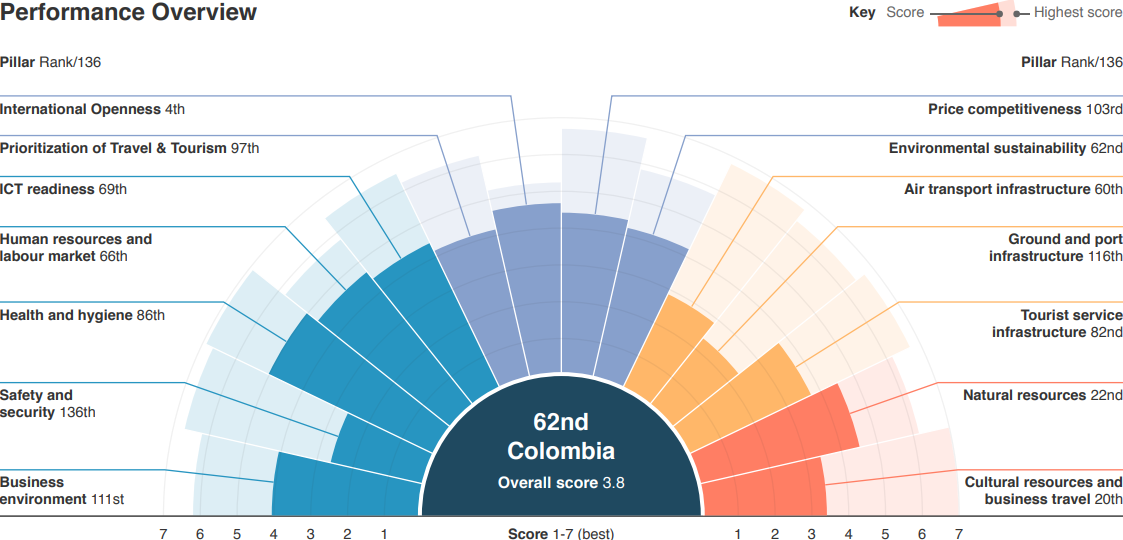
\includegraphics[width=6in]{wef.pdf}\centering
\caption{\label{wefAS}World Economic Forum report 2017 from \url{https://www3.weforum.org/docs/WEF_TTCR_2017_web_0401.pdf}.}
\end{figure}

%wef pillar13 nat res 22nd
Colombia % is a wonderful place, it
has everything: Pacific, Caribbean, jungle,
desert, mountains, you name it,  like Latin America in one country.
 So it is striking that according to WEF
in terms of Prioritization of Travel \& Tourism Colombia ranks 97th out of 136
countries \citep{world2017travel}. Its air transport infrastructure
is good, 60th, but Ground and Port Infrastructure is poor, 116th. But the worst
is Safety and Security, 136th/136. Surely Colombia should work to improve safety, but much
progress has already been done, and it is important to point out that much of
the country is safe, and dangerous Colombia is more of a stigma of the past than
present reality. 

USNEWS measures QOL as: A good job market, Affordable, Economically stable,
Family-friendly, Income equality, Politically stable, Safe, Well-developed
public education system, Well-developed public health system--see \url{https://www.usnews.com/news/best-countries/colombia}.

 
 % \section{Variables' definitions, coding, and distributions}
 % \label{app_var_des}


% %\input{/tmp/a.tex} %aok_var_des

% % \begin{spacing}{.9}
% %   \begin{table}[H]\centering \caption{Summary statistics.} \label{sumSta} \begin{scriptsize} \begin{tabular}{p{1.8in}p{.5in}p{.5in}p{.5in}p{.5in}p{.5in}p{.5in}p{.5in}p{.5in}p{.5in}p{.5
% %             in}p{.5in}p{.5 in}}\hline
% %         \input{/tmp/aha2.tex}
% %          \end{tabular}\end{scriptsize}\end{table}
% % \end{spacing}

% % \begin{spacing}{.9}
% %   \begin{table}[H]\centering \caption{Correlation matrix.} \label{sumSta} \begin{scriptsize} \begin{tabular}{@{}
% %           p{1.2in} rrrrrrrrrrrrr @{}}\hline
% %         \input{/tmp/ahb2.tex}\hline
% %          \end{tabular}\end{scriptsize}\end{table}
% % \end{spacing}



% Table XXX shows variable distributions. If a variable has more than
% 10 categories it is classified into bins...

% \input{../tmp/hist.tex}

 % \section{Additional Descriptive Statistics}
 % \label{app_des_sta}

% %make sure i have [H] or h! ???
% % \begin{table}[H]
% % \caption{}
% % \centering
% % \label{}
% % \begin{scriptsize}
% % \input{../out/reg_c.tex}
% % \end{scriptsize}
% % \end{table}

% \section{Additional Information}

% \ref{ingle}

% \begin{figure}[h!]
% \begin{centering}
% %\fbox{
%  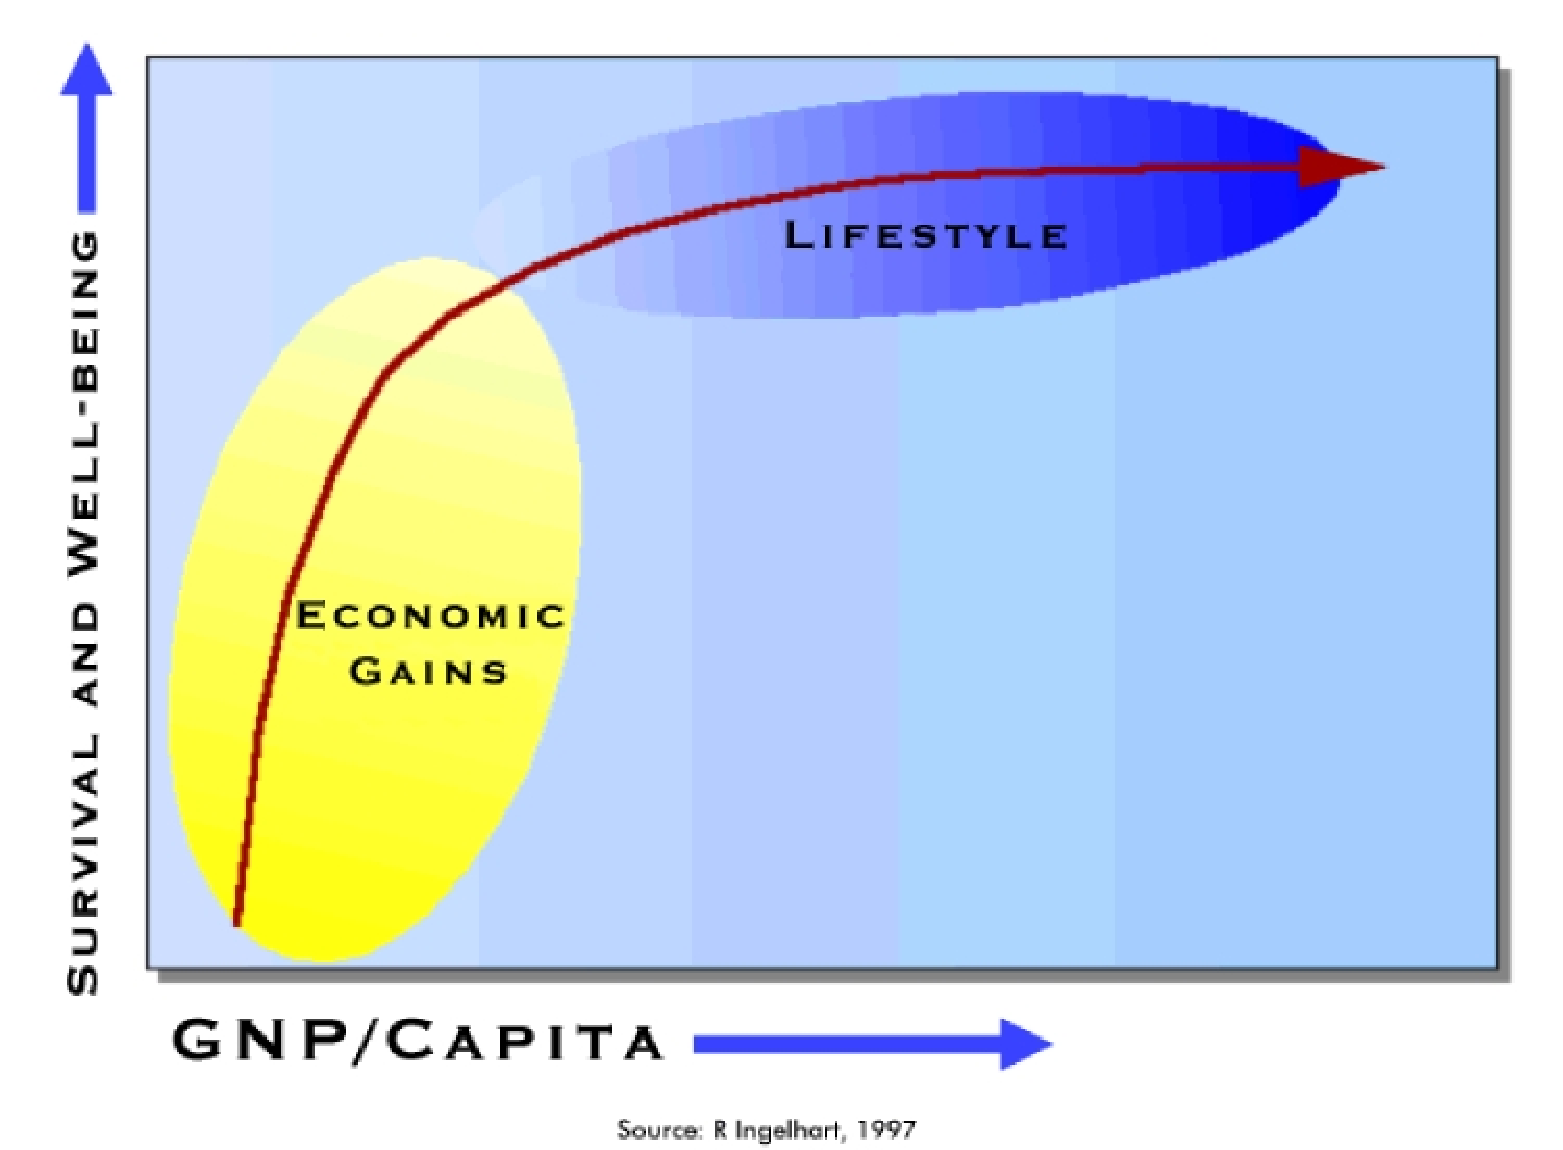
\includegraphics[height=2.5in]{/home/aok/papers/root/old/2011/eurostat_cities/tex/ingle.pdf}
% %} 
%  \caption{Well-being and income, \citep{inglehart97}.} \label{ingle}
%   \end{centering}
% \end{figure}


% TO n org
% later can redo with latinobarometer, goes back every year to like 95, but at
% least since 05 has 8 step urbanicity, but top one is 100k and then there is capital
% ad

% and then can do size with province :)




 
% \begin{figure}[H]
%  \includegraphics[height=3in]{record.pdf}\centering\label{record}
% \caption{Long term GDP from Colombian government.}
% \end{figure}


% \begin{spacing}{.9} \begin{table}[H]\centering   \begin{scriptsize} \begin{tabular}{p{1.8in}p{.5in}p{.5in}p{.5in}p{.5in}p{.5in}p{.5in}p{.5in}p{.5in}p{.5in}p{.5 in}p{.5in}p{.5 in}}\hline \input{reg-base.tex} \hline + 0.10 * 0.05 ** 0.01 *** 0.001; robust std err \end{tabular}\end{scriptsize}\caption{\label{a}OLS regressions of satisfaccionvida. See coef on 2018--they're becoming less happy!!}\end{table} \end{spacing}





\section{Freedom is Even The National Motto (Liberdad y Orden)}

\begin{figure}[H]
 \includegraphics[width=3in]{freedom.pdf}\centering\label{freedom}
\caption{Liberdad y Orden.}
\end{figure}

In the US despite all the hype about freedom, the motto is ``In God We Trust.''
Or the older version, ``E pluribus unum'' refers to being united, not
necessarily free. 



 \section{
 Dissociation}
% dan hart
% guess like this:
% https://www.mind.org.uk/information-support/types-of-mental-health-problems/dissociation-and-dissociative-disorders/about-dissociation/

% dan's student: Michaela Ancelo


%\section{Brief Definitions}

The words in this section could be used as measures.

$Amnesia <-$c("how did I get here", "brain is on autopilot", "when did I get changed", "where did this come from",
            "they say they know me", "they said they know me", "I don't recognize them", "stressful events causing memory loss",
            "I don't think I lied", "I know I didn't lie", "what did I do earlier", "gaps in my memory", "memory lapse",
            "lapse in memory", "who am I", "what were we talking about", "what are we talking about", "coming to", "I can't remember",
            "I cannot remember", "I don't remember", "I do not remember", "frustrated with my memory", "I wish I could remember",
            "I want to remember", "I look different", "I don't remember attempting suicide", "I don't remember hurting myself")


$Daydreaming <-$ c("inner self dialogue", "inner dialogue", "unable to recall the conversation", "confusing dreams with reality", "did that really happen",
                 "or was it a dream", "the world ceased to exist", "nothing around me matters", "my daydreams feel real",
                 "my fantasies feel real", "confusing my imagination with reality", "staring off", "not knowing time had passed",
                 "talking to myself aloud", "talking to myself out loud", "spaced out", "spacey", "floating off", "drifting off",
                 "I'm scattered", "I am scattered", "my mind is scattered", "my brain is scattered", "scatterbrained", "I'm all over the place",
                 "mentally all over the place", "mentally all over", "I'm not focused", "I am not focused", "I can't focus", "I cannot focus",
                 "my mind wandering", "I forgot my plans", "I forgot to do chores", "I forgot", "I forget", "daydreaming", "daydreams",
                 "blocking my memories", "blocked memories")

$Highway\_Hypnosis$ <- ("zoning out while driving")

$Absorption <-$ c("I lost all awareness", "stuck in a trance", "unaware of my surroundings")

$Derealization <-$ c("nothing is real", "nobody is real", "no one is real", "I am not real", "I feel strange here",
                   "everything seems unclear", "brain fog", "going within to protect myself", "going within",
                   "retreat within to protect myself", "retreat within", "turning within to protect myself", "turning within",
                   "ground falling beneath me", "ground falling out under me", "suddenly everything seems strange",
                   "suddenly everything seemed strange", "suddenly everything was strange", "everything seems foreign",
                   "everything seemed foreign", "everyone seems foreign", "everything seemed foreign", "I'm back at that place",
                   "reliving that moment", "reliving what happened", "flashbacks are debilitating", "debilitating flashbacks")

$Depersonalization <-$ c("debating myself", "their voice in my head", "familiar voice in my head", "their voices questioning me",
                      "other's voices nagging me", "looking at myself as another", "disconnected from myself", "feeling outside of my body",
                      "watching myself from the outside", "I don't recognize myself", "who is in the mirror", "this body isn't mine", "my body isn't mine",
                      "body doesn't belong to me", "I couldn't feel the pain", "ignore the pain", "I don't feel like myself", "I don't act like myself",
                      "it was unlike me", "I'm beside myself", "I am beside myself", "I'm not myself", "I am not myself", "I lost myself", "let go of myself",
                      "why did I do that", "what could've possessed me", "I wasn't myself", "I was not myself", "can't reveal my true self", "out of my mind",
                      "out of my head", "out of my skull", "being with myself", "my body isn't real", "my body is not real", "I am speaking another's words",
                      "why did I say that", "these thoughts aren't mine", "thoughts that aren't mine", "I'm not all there", "I am not all there",
                      "feeling empty and painfully alone", "feeling empty", "feelings of emptiness", "felt empty", "painfully alone", "feeling alone",
                      "felt alone", "I feel like a machine", "I feel like a robot", "I'm going through the motions", "going through the motions",
                      "I feel detached", "I felt detached", "I'm feeling detached", "I am feeling detached", "I was feeling detached",
                      "detached from myself", "why can't I move", "I feel paralyzed", "I felt paralyzed", "I watch myself", "I'm watching myself",
                      "I am watching myself", "I watched myself", "I was watching myself", "going through the motions", "watch myself going through life",
                      "watched myself going through life", "watching myself going through life", "watched myself complete daily tasks",
                      "watch myself completing daily tasks", "watching myself complete daily tasks", "my mind is empty", "my mind was empty",
                      "my mind is blank", "my mind was blank", "blank stare", "staing blankly", "stared blankly", "I seem gone")

$Identity\_Fragmentation <-$ c("mental conversations with myself", "conversations with myself", "inner back and fourth dialogue", "internal dialogue",
                          "I am two different people", "I'm two different people", "I was two different people", "like I was someone else",
                          "the voices in my head", "I'm at war with myself", "at war with myself", "fighting a war within", "I'm struggling with myself",
                          "I am struggling with myself", "struggling with myself", "that wasn't me", "that was not me", "nobody knows the real me",
                          "myself on the inside", "the real me", "know the real me", "talking things over with myself", "talking with myself",
                          "this feeling isn't mine", "this feeling is not mine", "feeling doesn't belong to me", "child's voice in my head",
                          "another personality taking over", "another personality controlling me", "why did I think that", "why would I think that",
                          "random thoughts", "intrusive thoughts", "sadness out of nowhere", "strong feelings out of nowhere", "filled with pain",
                          "resist the urge", "these urges aren't mine", "urges are not mine", "feeling split or divided", "feeling split inside",
                          "felt split inside", "feeling divided inside", "feel divided inside", "felt divided inside", "is this really me",
                          "is this who I am", "inability to keep friends", "I can't keep friends", "I cannot keep friends", "I feel different than normal",
                          "I felt different", "I'm feeling different than normal", "was different than normal", "I feel weird", "I felt weird", "I'm feeling weird",
                          "I was feeling weird", "I feel strange", "I felt strange", "I'm feeling strange", "I am feeling strange", "I was feeling strange", "I feel odd",
                          "I felt odd", "I'm feeling odd", "I am feeling odd", "I was feeling odd", "voices saying to hurt myself", "the voices say hurt yourself",
                          "my head is too loud", "my head is so loud", "my head was so loud", "inside my head is loud", "inside my head was loud",
                          "screaming inside my head", "screams inside my head", "yelling inside my head", "noise inside my head", "angry out of nowhere",
                          "why am I angry", "filled with anger", "I have multiple personalities", "I have many personalities", "I don't feel whole",
                          "I do not feel whole", "I am not whole", "I'm not whole", "part of me is missing", "missing a part of myself", "racing thoughts",
                          "my thoughts are racing", "my thoughts were racing", "racing mind", "my mind is racing", "my mind was racing", "can't stop racing thoughts",
                          "cannot stop racing thoughts", "thoughts won't stop racing", "thoughts will not stop racing", "I can't stop thinking",
                          "I cannot stop thinking", "I want to stop thinking", "struggling with my identity", "struggling to find my identity",
                          "struggling with who I am", "figuring out who I am", "acting like another person", "I am not that person", "I'm not that person",
                          "unlike myself", "protective voice in my head", "helpful voice in my head", "soothing voice in my head")





\end{spacing}
\end{document}




sth wrong my wvs shows ls flat and ruut veenhoven shows huge growth (but his conversion to 1-10 doesn't, so maybe his 1-10 is right lol) and hist first measure (wvs!) on page https://worlddatabaseofhappiness-archive.eur.nl/hap_nat/desc_na_genpublic.php?cntry=122 shows 3.3 in 1998!!
%table centered on decimal points:)
\begin{table}[H]\centering\footnotesize
\caption{\label{t1} Colombia's happiness on scale 1-4 over time and on
  scale 1-10 across space (23 happiest countries in the world) . Data from World Database of Happiness at \url{https://worlddatabaseofhappiness-archive.eur.nl/hap_nat/desc_na_genpublic.php?cntry=122}, originally from \citet{graham02,graham01,graham05} and Latinobarometro.}
\begin{tabular} {@{} lr||rrrrrr @{}}   \hline 
year& Colombian happiness (1-4) &happiness rank& country& happiness (1-10) \\ \hline
1997&2.5    & 1 	&	Denmark	        &	8.2      \\                          
2000&2.4    & 2 	&	Mexico	        &	8.1      \\                          
2001&3.06   & 3 	&	Colombia	&	8.1      \\                  
2003&3.16   & 4 	&	Switzerland	&	8        \\                  
2004&3.14   & 5 	&	Finland	        &	8        \\                          
2004&3.45   & 6 	&	Iceland	        &	8        \\                          
2005&3.17   & 7 	&	Costa Rica	&	7.9      \\                  
2005&3.36   & 8 	&	Norway	        &	7.9      \\                          
2006&3.25   & 9 	&	Canada	        &	7.9      \\                          
2006&3.4    & 10	&	Qatar         	&	7.8      \\                          
2007&3.36   & 11	&	Sweden	        &	7.8      \\                          
2008&3.39   & 12	&	Austria    	&	7.7      \\                          
2009&3.3    & 13	&	Nicaragua	&	7.7      \\                  
2009&3.4    & 14	&	Uzbekistan	&	7.7      \\                  
2010&3.46   & 15	&	Netherlands	&	7.6      \\                  
2010&3.18   & 16	&	Ecuador  	&	7.6      \\                          
2011&3.22   & 17	&	Israel  	&	7.6      \\                          
2013&3.3    & 18	&	Luxembourg	&	7.6      \\                  
2015&3.3    & 19	&	Belgium 	&	7.5      \\                          
2016&3.28   & 20	&	United Arab Emirate&	7.5      \\               
2017&3.34   & 21	&	Bosnia Herzegovina &	7.5      \\               
2018&3.35   & 22	&	Panama  	&	7.5      \\                          
2020&3.37   & 23	&	Brazil  	&	7.4      \\\hline                    
\end{tabular}\end{table}       



big change 50perc change in trust, and small about 3perc in freedom;

in addition to key SWB, we also look at two additional subjective wellbeing
indicators, trust and freedom (SEE MY ERALIER PAPERS ON TRUST AND FREEDOM--what
control for)

rt super interesting, swb flat; but trust went down a lot to a mere .05!! makes
sense all the politics and unrest; but freedom if anything went up, indeed as
some protesters would often say ``we're not afraid anymore''


trust and freedom for later; just swb
. tabstat trust,  stat(count mean sd) by(yr) format(%9.2f)
tabstat trust,  stat(count mean sd) by(yr) format(%9.2f)

Summary for variables: trust
     by categories of: yr (Year survey)

    yr |         N      mean        sd
-------+------------------------------
  1997 |   2995.00      0.10      0.31
  1998 |   2986.00      0.11      0.32
  2005 |   2993.00      0.14      0.35
  2012 |   1501.00      0.04      0.20
  2018 |   1520.00      0.05      0.21
-------+------------------------------
 Total |  11995.00      0.10      0.30
--------------------------------------

. tabstat freedom,  stat(count mean sd) by(yr) format(%9.2f)
tabstat freedom,  stat(count mean sd) by(yr) format(%9.2f)

Summary for variables: freedom
     by categories of: yr (Year survey)

    yr |         N      mean        sd
-------+------------------------------
  1997 |      0.00         .         .
  1998 |   2996.00      7.89      2.09
  2005 |   3002.00      8.04      2.20
  2012 |   1507.00      8.16      1.96
  2018 |   1520.00      8.12      2.31
-------+------------------------------
 Total |   9025.00      8.02      2.15
--------------------------------------
